\documentclass{article}
\usepackage{amsmath}
\usepackage{amssymb}
\usepackage{amsfonts}
\usepackage{multirow}
\usepackage{graphicx}
\usepackage{array}
\graphicspath{ {/home/poiso/uni/primo-anno/Matematica-Discreta-1/} }
\title{Matematica Discreta}
\begin{document}
    \section{Prima parte}
    \begin{flushleft}

    \end{flushleft}
    \section{Numeri}
    \subsection{Principio di Induzione}
    \begin{flushleft}
        In matematica esistono 3 diversi modi per dimostrare
        $A\to B$
        \begin{enumerate}
            \item Dimostrazione Diretta
            \item Dimostrazione per assurdo
            \item Principio di induzione matematica
        \end{enumerate}
        \subsubsection{Esempio}
        \begin{equation}
            \sum_{i=0}^n i = \frac{(n+1)n}{2}
            \label{eq:1 }
        \end{equation}
        \textbf{Passo Base}\\
        \begin{equation}
            \sum_{i=0}^1 i = \frac{(1+1)1}{2} = 1
            \label{eq:2 }
        \end{equation}
        \textbf{Passo Induttivo}\\
        Supponiamo vera P(m) per $\forall m<n$
        \begin{equation}
            \sum_{i=0}^n i = \sum_{i=0}^{n-1} i+n= \frac{(n+1)n}{2} +n = n(\frac{n-1}{2} +n)=\frac{(n+1)n}{2}
            \label{eq: 3}
        \end{equation}
        Pertanto n e' vera $\forall n \in \mathbb{P}$
    \end{flushleft}
    \subsection{Il principio del buon ordinamentoa (WOP)}
    \begin{flushleft}
            $S \subseteq \mathbb{Z}$ allora $\rightarrow \exists m\in S$ tale che $m\leq x$ per $\forall x\in S$
    \end{flushleft}
    \begin{flushleft}
        \textbf{Osservazione:} Falso per $\mathbb{Z} (S = \{-1,-2,-3\}$ non ha il minimo
    \end{flushleft}
    \subsection{Numeri Positivi,Interi e razionali}
    \begin{flushleft}
       Questi Insiemi numerici li abbiamo gia definiti all inizio degli appunti.
        Equivalenza di $\mathbb{Z} x (\mathbb{Z} / \{0\})$
    \end{flushleft}
    \subsection{Numeri Reali}
    \begin{flushleft}
    Si veda il corso di analisi. Intuitivamente i numeri reali sono le lunghezze dei segmenti.
    \end{flushleft}
    \subsection{Numeri Primi e composti}
    \begin{flushleft}
        Sono $a,b\in \mathbb{P}$\\
        Definizione: si dice che a divide b ( o che b e' multiplo di a) se $\exists k \in \mathbb{Z}$ tale che $b=k*a$
        \textbf{Osservazioni}
        \begin{itemize}
            \item $a|b \rightarrow a\leq b$
            \item $a|b \land b|c \rightarrow a|c$
            \item $a|b \land a|c \rightarrow a|(xb+yc) \forall x,y\in \mathbb{Z}$
        \end{itemize}
        Definizione: sia $a\in \mathbb{P}$, a si dice primo se $b|a \rightarrow b=1 \lor b=a \land a\geq 2$ altrimeenti a si dice composto \\
        Siano $a,b\in \mathbb{P}$ si dicono coprimi (o primi tra loro) se:
        \begin{equation}
            c|a \land c|b \rightarrow c=+-1
        \end{equation}
        \textbf{Osservazione:} $p_1$ e $p_2$ primi, $p_1 \neq p_2 \rightarrow$ $p_1$ e $p_2$ sono coprimi\\
       Definzione: a si dice perfetto se a e' uguale alla somma dei suoi divisori.
       \begin{itemize}
           \item 6 e' perfetto (1+2+3=6)
           \item 8 non e' perfetto (1+2+4 $\neq$ 8)
       \end{itemize}
    \end{flushleft}
    \subsubsection{Teorema}
    \begin{flushleft}
        Sia $n\in \mathbb{P}$ allora o n e' primo o n e' prodotto di primi. \\
        \textbf{Dimostrazione} Induzione completa, se n=2 e' un numero primo supponiamo che il Teorema
        sia vero per $\forall m \in \mathbb{P}$ $2 \leq m \leq n$
        \begin{itemize}
            \item Se n e' primo ok
            \item se non e' primo $\rightarrow \exists a,b \in \mathbb{P}$ tali che n=n*b
                ma per induzione , a e b sono o primi o prodotti di primi $\rightarrow $ n allora e' prodotto di primi
        \end{itemize}
    \end{flushleft}
    \subsubsection{Teorema}
    \begin{flushleft}
      Ci sono infiniti numeri primi: \textbf{Dimostrazione} per assurdo. Supponiamo che ci siano un numero finito di numeri primi $\{p_1,p_2,...,p_n\}$ 
      \begin{equation}
       N = p_1*p_2*...*p_n+1 
      \end{equation}
      Allora come dimostrato in 2.5.1 N e' prodotto di numeri primi per tanto $\exists q \in \mathbb{P}$, q e' primo, tale che q|N. \\
      Allora $q\notin \{p_1,...,p_n\}$. Se $q=p_1$ $\to$ $q|p_1$ e $q|N$ $\to$ $q|p_1,....p_n$ e q|N $\to$ $q|(N-p_1*p_2*...*p_n)$ $\to$ q|1 cioe' $q\leq1$ e quindi assurdo
      se $q\geq2$ similmente avremmo che: $q=p_2,q=p_3$, etc.
    \end{flushleft}
    \subsubsection{Teorema (Hadamard-De la valle poussin}
    \begin{flushleft}
      \begin{equation}
        \lim_{n \to \infty} \frac{\pi(n)}{\frac{n}{ln(n)}} =1
      \end{equation}
    \end{flushleft}
    \subsection{Algoritmo Euclide}
    \begin{flushleft}
      Siano $a,b\in \mathbb{P}$ \\ 
      \textbf{Definizione}: il massimo comune divisore di a e b, scritto: MCD(a,b) (o GCD(a,b)) e':
      \begin{equation}
        c = max\{ n \in \mathbb{P}: n|a \land n|b \} 
      \end{equation}
      Come calcolare MCD(a,b)? \\ 
    \end{flushleft}
    \subsubsection{Lemma}
    \begin{flushleft}
      Siano $a,b \in \mathbb{P}$ , $a\geq b$. Allora $\exists q,r \in \mathbb{Z}$ tali che a=bq+r e $0\leq r <b$ \\ 
      \textbf{Dimostrazione:} e' nota
      \textbf{Agoritmo Euclideo}\\       
      Siano $a,b \in \mathbb{P}$, $a\geq b$. Allora $\exists q,r \in \mathbb{Z}$ tali che a=bq+r e $0\leq r <b$ \\
      Se $r=0$ $\to$ MCD(a,b)=b \\ 
      Se $r>0$ $\to$ $\exists  q,r \in \mathbb{Z}$ tali che $b=q_1*r+r_1$ e $0\leq r_1 <r$
      Se $r_1=0$ $\to$ MCD(a,b)=r \\ 
      Se $r_1>0$ $\to$ $\exists  q_2,r_2 \in \mathbb{Z}$ tali che $b=q_2*r_1+r_2$ e $0\leq r_2 <r_1$
      Se $r_2=0$ $\to$ MCD(a,b)=$r_1$ \\ 
      Se $r_2>0$ $\to$ $\exists  q_3,r_3 \in \mathbb{Z}$ tali che $b=q_3*r_2+r_3$ e $0\leq r_3 <r_2$ etc... \\ 
      In questo modo si ottiene una sequenza di numeri $b>r>r_1>r_2>...\geq 0$ \\ 
      $\exists k \in \mathbb{P}$ tale che $r_k=0$. L'algoritmo termina allora MCD=$r_{k-1}$ \\ 
      \textbf{Perche' funziona?} \\ 
      L'Algoritmo di Euclide produce due sequenze di numeri $r_1,r_2,r_3...$ e $q_1,q_2,q_3...$ tali che
        \begin{equation}
           a = bq +r  
           b= q_1*r+r_1  
           r_i = q_{i+2}*r_{i+1} + r_{i+2} % da allineare
        \end{equation}
        Sia $k\in \mathbb{P}$ tali che $r_k=0$. Ma
        \begin{equation}
          r_{k-2}=q_k*r_{k-1} + r_k \to r_{k-1}|r_{k-2} 
        \end{equation}
        \begin{equation}
          r_{k-3}=q_{k-1}*r_{k-2} + r_{k-1} \to r_{k-1}|r_{k-3} 
        \end{equation}
        \begin{equation}
          b=q*r+r_1 \to r_{k-1}|b \quad \quad a=b*q+r\to r_{k-1}|a 
        \end{equation}
        Quindi $r_{k-1}$ e' un divisore comune di a e b
        \\
        Sono $a,b \in \mathbb{P}, a\geq b$ L'algoritmo di Euclide produce due sequenze di numeri $q_1,q_2...$ e $r_1,r_2,...$ $\in \mathbb{Z}$ tali che 
        \begin{itemize}
          \item $a=bq+r$
          \item $b=q_1r+r_1$
          \item $r_i=q_{i+2}r_{i+1}+r_{i+2}$
        \end{itemize}
        Sia $r_k=0$ Sia $c\in \mathbb{P}$ tali che c|b e c|a. Ma allora c|r(=a-bq) $\Rightarrow$ c|$r_1$ (= b-$q_1$r)$\Rightarrow$ c|$r_i$ per
        $\forall i=1,...,k-2$ Pertanto $2_{k-1}$=MCD(a,b)
        E.g \\ 
        Calcolare il massimo comune divisore (153,126), Applichiamo l algoritmo:
        $153=1*126+27$ \\ 
        $126=4*27+18$ \\
        $27=1*18+9 \Rightarrow$ 9 e' il nostro massimo comune divisore \\
        $18=2*9+0$ \\
    \end{flushleft}
    \subsection{Conseguenze dell Algoritmo di Euclide}
    \begin{flushleft}
     Siano a,b,q,r come in A.E  \\ 
      \textbf{Osservazione:} Se $r>0 \Rightarrow$ MCD(a,b)=MCD(b,r)
    \end{flushleft}
    \subsubsection{Identita' di Bezout}
    \begin{flushleft}
      Siano $a,b \in \mathbb{P}.$ Allora $\exists x,y \in \mathbb{Z}$ tali che
      \begin{equation}
        (a,b)=ax+by
      \end{equation}
      Dimostrare sia $a\geq b$. Induzione completa su $b\geq 1$. \\ 
      \textbf{Passo base} \\ 
      Se b=1 $\Rightarrow$ b|a $\Rightarrow$ (a,b) = b $\Rightarrow$ a*0+b*1 $\Rightarrow$ ok \\
      Supponiamo la tesi vera per tutti i numeri $<b$.Allora $\exists q,r \in \mathbb{Z}$ tali che a=bq+r e $0\leq r < b$.
      \begin{itemize}
        \item Se $r=0$ $\Rightarrow$ b|a $\Rightarrow$ (a,b) = b $\Rightarrow$ ok
        \item Se $r>0  \Rightarrow (a,b)=(b,r).$ Ma $r<b \Rightarrow_{induzione} \exists x,y \in \mathbb{Z}$ tali che: $(b,r)=bx+2y$
      \end{itemize}
      Ma allora
      \begin{equation}
        (a,b)=bx+2y=bx+(a-b*q)y=b(x-qy)+ay. \square
      \end{equation}
    \end{flushleft}
    \subsubsection{Proprieta}
    \begin{flushleft}
      Siano $a,b \in \mathbb{P}$. Allora
      \begin{equation}
        (a,b)=min\{ax+by \in \mathbb{P}:x,y \in \mathbb{Z}\}
      \end{equation}
    \end{flushleft}
    \subsubsection{Proprieta}
    \begin{flushleft}
      Siano $a,b,p \in \mathbb{P}$ \\ 
      p primo tale che p|ab. Allora p|a o p|b.
      \textbf{Dimostrazione}: 
      \begin{itemize}
        \item Se p|a $\Rightarrow$ ok \\ 
        \item Se p not| a $\Rightarrow$ a,p=1 $\Rightarrow$ c|p $\Rightarrow$ c|a e c=1 o c=p
      \end{itemize}
      $\exists x,y \in \mathbb{Z}$ tali che 1=ax+py $\Rightarrow$ b=abx+pby $\Rightarrow$ p|b $\square$
      \textbf{Osservazioni}
      \begin{itemize}
        \item Falsa in generale se p non e' primo
        \item Analogamente si dimostra che se $m,a,b \in \mathbb{P}$ allora m|ab e (m,a)=1 $\Rightarrow$ m|b
      \end{itemize}
    \end{flushleft}
    \subsubsection{Teorema Fondamentale dell' Aritmetica}
    \begin{flushleft}
      Sia $n\in \mathbb{P}$. Allora n non puo' essere espresso in uno ed un solo modo come prodotto di numeri primi , a parte l'ordinamento dei fattori\\ 
      \textbf{Dimostrazione}:se $n \geq 2$. Sia n=2 e siano $p_1,p_2$ primi tali che $2=p_1*p_2 \Rightarrow p_1 \mid 2 \Rightarrow p_1 \leq 2 \Rightarrow p_2 = 2$
      \begin{equation}
       n=p_1*...*p_2=q_1*...*q_2 
      \end{equation}
      Allora $p_1 \mid m \Rightarrow p_1 \mid q_1*...*q_s \Rightarrow \exists 1\leq i < s : \quad p_1 \mid q_i \Rightarrow p_1=q_i$\\ 
      Ma allora
      \begin{equation}
        \frac{n}{p_1}=p_2*...*p_r=q_1*...*q_{i-1}*...q_s 
      \end{equation}
      ma $\frac{n}{p} < n \Rightarrow $ le due fattorizazioni coincidono a meno dell'ordine dei fattori, anche quelli in (15) coincidono a numeri
      dell'ordine dei fattori $\square$.
    \end{flushleft}
    \subsection{Equazione Diofane lineare}
    \subsubsection{Teorema}
    \begin{flushleft}
     Allora $\exists x,y \in \mathbb{Z}$ tali che
     \begin{equation}
       ax+by=n \quad (\square)
     \end{equation}
     se e solo se $(a,b) \mid h$\\ 
     \textbf{Dimostrazione}: Se $\exists x,y \in \mathbb{Z}$ tale che la formula vale, poiche' $(a,b)\mid a$ e $(a,b) \mid ab$ $\Rightarrow$ $(a,b)\mid h$\\ 
     Viceversa se $(a,b)\mid n \Rightarrow \exists k \in \mathbb{Z}: \quad n=k(a,b)$ Ma per 2.7.1 $\Rightarrow \exists x,y \in \mathbb{Z}$ tale che
     \begin{equation}
       ax+by=(a,b)
     \end{equation}
      Quindi axk + byk=n $\square$
    \end{flushleft}
    \subsubsection{Teorema}
    \begin{flushleft}
      Siano $a,b \in \mathbb{P}$. Allora le soluzioni $x,y \in \mathbb{Z}$ di ax+by=n sono tutte (se esistono, cioe' se $(a,b)\mid n$) della forma \\
      \begin{equation}
        \begin{cases}
          x= x_0 - \frac{b}{(a,b)}t \\
          y= y_0 - \frac{a}{(a,b)}t
        \end{cases}
      \end{equation}
      se hai una soluzione di una delle 2 equazioni puoi ricavare l altra.
      \\ 
      Doce $t \in \mathbb{Z} \quad x_0,y_0 \in \mathbb{Z}$ e' una soluzione di ($\square$).
    \end{flushleft}
     \subsection{Le classi di resto} 
     \begin{flushleft}
       Sia $n \in \mathbb{P}$. Poniamo una relazione $\equiv_n$ su $\mathbb{Z}$ in questo modo
       \begin{equation}
         a \equiv_n b \iff n\mid (b-a)
       \end{equation}
       $\forall a,b \in \mathbb{Z} \quad "\equiv_n"$ si dice "relazione di congruenza modulo n"( si scrive anche $a \equiv b(modn)$
     \end{flushleft}
     \subsubsection{Proprieta}
     \begin{flushleft}
       $\equiv_n$ e' di equivalenza. Dimostrazione: vedi 1.4 (n=3) $\square$\\ 
       Le classi di equivalenza rispetto $a \equiv_n$ si dicono classi di resto (modulo n), scritto $[a]_n$.E.g
       \begin{equation}
         \begin{split}
           [6]_8 & = \{6,14,-2,22,-10,...\}\\
           & = \{ b\in \mathbb{Z}:b \equiv_8 6 \}
         \end{split}
       \end{equation}
       Ci sono n classi di resto modulo n e cioe' $[0]_n,[1]_n...[n-1]_n$ \\ 
       Oss: Siano $a,b,c,d \in \mathbb{Z}$ e $n \in \mathbb{P}$ allora
       \begin{equation}
         a \equiv_n c \land b\equiv_n d \Rightarrow a+b \equiv_n c+d
       \end{equation}
       \begin{equation}
         a \equiv_n c \land b\equiv_n d \Rightarrow ab \equiv_n cd
       \end{equation}
       Ci suggerisce le seguenti definizioni.
       Poniamo 
       \begin{equation}
         [a]_n + [b]_n =^{def} [a+b]_n
       \end{equation}
       \begin{equation}
         [a]_n * [b]_n =^{def} [ab]_n
       \end{equation}
       (Somme e prodotto di classi di resto)\\ 
       Le classi di resto si comportano come numeri tranne quando:
       \begin{equation}
        [a]_n * [k]_n = [b]_n * [k]_n \land [k]_n \neq [0]_n
       \end{equation}
       questo non implica $[a]_n = [b]_n$ \\ 
       E.g
       \begin{equation}
         [6]_8 [4]_8 = [2]_8 [4]_8 \land [4]_8 \neq [0]_n
       \end{equation}
        ma $[2]_8 \neq [6]_8$
     \end{flushleft}
     \subsubsection{Proprieta}
     \begin{flushleft}
      Siano $a,b,k \in \mathbb{Z}$ e $n \in \mathbb{P}$ tali che (n,k)=1. Allora
       \begin{equation}
        [a]_n*[k]_n=[b]_n*[k]_n \Rightarrow [a]_n=[b]_n 
       \end{equation}
       Dimostrazione: Abbiamo che \\
       $[ak]_n=[bk]_n \Rightarrow a*k=b*k \Rightarrow n\mid k(b-a) \Rightarrow_{(n,k)=1}n\mid (b-a) \Rightarrow a \equiv_n b \Rightarrow [a]_n \equiv [b]_n \square$
     \end{flushleft}
     \begin{flushleft}
       Siano $a \in \mathbb{Z}$ e $n \in \mathbb{P}$ \\ 
       Definizione: un' inversa moltiplicativa di $[a]_n$ e' una $[b]_n$ tale che:
       \begin{equation}
         [a]_n*[b]_n=1
       \end{equation}
     \end{flushleft}
     \subsubsection{Proprieta}
     \begin{flushleft}
       Siano $a \in \mathbb{Z} \quad n \in \mathbb{P}$ tali che (a,n)=1. Allora $\exists ! [b]_n$ tale che
       \begin{equation}
         [a]_n*[b]_n=[1]_n
       \end{equation}
       \textbf{Dimostrazione:}Per Bezout $\Rightarrow \quad \exists x,y \in \mathbb{Z}: ax+by=1 \Rightarrow [a]_n*[x]_n = [ax]_n=[1-ny]_n=[1]_n$ \\ 
       Sia $[y]_n$ tale che $[a]_n*[y]_n=[1]_n$. Allora $[a]_n *[x]_n=[a]_n*[y]_n \to$ per 2.9.2 $\to [x]_n=[y]_n \square$
     \end{flushleft}
     \subsection{Le funzioni di Eulero}
     \begin{flushleft}
       \begin{equation}
         \Phi (n)=\mid \{ i\in \mathbb{P}: 1 \leq i \leq n, (n,i)=1\}\mid
       \end{equation}
       E.g
       \begin{equation}
         \Phi (8) =4.
       \end{equation}
       Osservazione $p\in \mathbb{P}$, p primo $\Rightarrow \Phi (p)=p-1$
     \end{flushleft}
     \subsubsection{Proprieta}
     \begin{flushleft}
      Siano p,q primi $p \neq q$. Allora 
       \begin{equation}
         \Phi (p*q)=(p-1)(q-1)
       \end{equation}
       \textbf{Dimostrazione:} Abbiamo che 
       \begin{equation}
         \Phi (p*q)=pq-\mid \{1 \leq i \leq pq : (pq,i) \geq 2\} \mid 
       \end{equation}
       Sia $r\in \mathbb{P}$, r primo allora:
       \begin{equation}
         r \mid i \land r \mid pq \iff r \mid i \land (r\mid p \lor r\mid q) \iff r\mid i \land (r=p \lor r=q)
       \end{equation}
       Quindi $p \mid i \lor q \mid i$ \\ 
       $i \in \{ p, 2p,3p,...(q-1)p,qp,q,2q,...(p-1)q\} \Rightarrow $ ci sono quindi p+q+1 tali i
     \end{flushleft}
     \subsubsection{Teorema}
     \begin{flushleft}
       Sia $n \in \mathbb{P}$ e sia $n = p^{a_1}_1*....*p^{a_r}_r$ la sua decomposizione in numeri primi:
       \begin{equation}
         \Phi (n) = n(1-\frac{1}{p_1})*...(1-\frac{1}{p_r})
       \end{equation}
        Dimostrazione vedi capitolo 3 $\square$ 
     \end{flushleft}
     \subsubsection{Con}
     \begin{flushleft}
       Siano $a,b \in \mathbb{P}$ tali che (a,b)=1. Allora:
       \begin{equation}
         \Phi (ab)=\Phi (a) * \Phi (b)
       \end{equation}
       Dimostrazione segue da 2.10.2 $\square$ \\ 
       Sia $n \in \mathbb{P}$. Poniamo
       \begin{equation}
         E_n = \{[i]_n: i\in \mathbb{Z} \quad (i,n)=1
       \end{equation}
      Notiamo che se $a,b \in \mathbb{Z}$ tali che $[a]_n=[b]_n$ allora:
       \begin{equation}
         (a,n)=1 \iff (b,n)=1
       \end{equation}
       Infatti, poiche' le classsi sono uguali $[a]_n=[b]_n \Rightarrow n \mid (b-a) \Rightarrow \exists k \in \mathbb{Z}$ tali che a=b+kn. Sia
       $r \in \mathbb{P}$, r primo. Allora
       \begin{equation}
        r\mid a \land r\mid n \iff r\mid b \land r\mid n
       \end{equation}
       Osservazione: $\mid E_n \mid = \Phi(n)$
     \end{flushleft}
     \subsubsection{Proprieta}
     \begin{flushleft}
       Siano $n \in \mathbb{P} \quad k \in \mathbb{Z}$ tali che (k,n)=1. Allora la funzione $f:E_n \to E_n$ definita da $f([i]_n)=[i]_n*[k]_n$ \\ 
       $\forall [i]_n \in E_n$ e' biunivoca
       Dimostrazione: Sia $[i]_n \in E_n \Rightarrow (i,n)=1 \Rightarrow [i*k]\in E_n \Rightarrow [i]_n*[k]_n \in E_n$ \\ 
       Siano $[i]_n[j]_n \in E_n $ tali che $ [i]_n*[k]_n=[j]_n*[k]_n \Rightarrow [i]_n = [j]_n$ quindi e inniettiva \\ 
       Sia $[a] \in E_n$ Poiche' (k,n)=1 $\Rightarrow \exists [b]_n \in E_n$ tali che \\ 
       $[k]_n*[b]_n =[1]_n$ Allora $[ab]_n \in E_n \Rightarrow [ab]_n*[k]_n=[a]_n[b]_n[k]_n= [a]_n*[1]_n=[a]_n \square $ e' surriettiva
     \end{flushleft}
     \subsubsection{Teorema di Eulero}
     \begin{flushleft}
       Siano $k \in \mathbb{Z}$ e $n \in \mathbb{P}$, tali che (n,k)=1 allora:
       \begin{equation}
         k^{\Phi(n)} \equiv_n 1 
       \end{equation}
     \end{flushleft}
     \begin{flushleft}
       Dimostrazione: Sappiamo da 2.10.4 che la funzione 
       \begin{equation}
         [a]_n \to [a]_n*[k]_n
       \end{equation}
       e' una biezione di $E_n$. Sia
     \end{flushleft}
     \begin{equation}
       E_n = \{ [k]_n,...,[k_r]_n\} \Rightarrow r=\Phi (n)
     \end{equation}
     \begin{flushleft}
      Dimostrazione sappiamo da 2.10.4 che ha funzione
       \begin{equation}
         [a]_n \to [a]_n*[k]_n
       \end{equation}
       e' una biezione di $E_n$. Sia
       \begin{equation}
         E_n = \{ [k]_n,....,[k_r]_n\} \Rightarrow r = \Phi (n)
       \end{equation}
       Ma allora:
       \begin{equation}
         E_n = \{ [k_1 * k]_n,....,[k_r * k_]n\} 
       \end{equation}
       Quindi:
       \begin{equation}
         [k_1]_n*...*[k_r]_n=[k_1]_n*...*[k_r]_n*[k]_n
       \end{equation}
       \begin{equation}
         [1]_n*[k_1]_n*...*[k_r]_n=[k_1]_n*...*[k_r]_n*[k]^r_n = [1]_n=[k^r]_n. \square
       \end{equation}
     \end{flushleft}
     \subsubsection{Teorema di Fermat-Eulero}
     \begin{flushleft}
       Siano $k \in \mathbb{Z}$ e $p \in \mathbb{P}$, primo, tale che $p \nmid k$ allora:
       \begin{equation}
         k^{p-1} \equiv_n 1
       \end{equation}
       Dimostrazione: Basta porre n=p in 2.10.5 $\square$
     \end{flushleft}
     \subsection{Il codice RSA}
     \begin{flushleft}
      Problema fondamentale della crittografia: \\ 
       Spedire un mesaggio da  A a B in modo che solo B possa leggerlo (decifrarlo).
     \end{flushleft}
     \begin{itemize}
       \item \textbf{Preparazione:} B sceglie 2 primi p e q, p $\neq$ q e calcola:
         \begin{equation}
          n=pq
         \end{equation}
         Quindi sceglie $e \in \mathbb{P}$ tali che 
         \begin{equation}
           (e,(p-1)(q-1))=1
         \end{equation}
         Infine calcola l'inversa moltiplicativa $[d]_{(p-1)(q-1)}$ di $[e]_{(p-1)(q-1)}$\\ 
         B pubblica n,e  e tiene segreti p,q,d
       \item \textbf{Codifica:} A prende un mesaggio $1 \leq m \leq n,(m,n)=1$ e calcola
         \begin{equation}
           [m^{\sim}]_n=[m^e]_n
         \end{equation}
         e spedisce $m^{\sim}$
       \item \textbf{Decodifica:} B riceve $m^{\sim}$ e decodifica calcolando
         \begin{equation}
           [m^{\sim d}]_n
         \end{equation}
     \end{itemize}
     \begin{flushleft}
       Osservazione: A e B non si scambiano niente. Perche pensiamo che sia difficile rompere RSA? Per rompere RSA dovremmo:
     \end{flushleft}
     \begin{itemize}
       \item Fattorizzare n ( caso impossibile se n e' grande)
       \item risolvere l equazione della forma:
         \begin{equation}
           [x^e]_n=[m^{\sim}]_n
         \end{equation}
     \end{itemize}
     \begin{flushleft}
      Se e=2 $\Rightarrow$ teoria della recipocita' quadratica \\ 
       Se e $\geq$ 3 $\Rightarrow$ ricerche attuali
     \end{flushleft}
     \begin{flushleft}
      Attualmente grande va a significare piu di 10000 cifre
     \end{flushleft}
     \subsubsection{Altri tipi di codici}
     \begin{itemize}
       \item Codice romano (Debolezza $\to$ analisi delle frequenza)
       \item Codice di Turing (Debolezza $\to$ $MCD(mp,m_1p_1,...)=p$
     \end{itemize}
     RECUPERARE LE LEZIONI
     \section{Combinatorie Enumerative}
     \subsection{Problema fondamentale della combinatoria enumerativa}
     \begin{flushleft}
       Data una sequenza di insiemi $\{A_n\}_{n \in \mathbb{N}}$, calcolare $\mid \{A_n\}_{n \in \mathbb{N}}\mid  $,
     \end{flushleft}
      Cosa vuol dire "calcolare"?
     \begin{enumerate}
      \item Una ricorsione (e.g $\mid A_n\mid = \mid A_{n-1} \mid + \mid A_{n-2} \mid$ se $n \geq 2$)
      \item Una formula (e.g $\mid A_n \mid = 2^n$)
      \item Una funzione generatrice (cioe' una funzione $f: \mathbb{R} \to \mathbb{R}$,$C^\infty$ in x=0, tale che lo sviluppo in serie di Taylor di f(x) in x=0 e'
        \begin{equation}
          \sum_{n\geq 0} \mid A_n \mid  x^n
        \end{equation}
      \end{enumerate}
      \subsection{Proprieta' Fondamentale}
      \begin{flushleft}
        Osservazione: A,B insiemi, $f:A\to B$ biunivoca
        \begin{equation}
          \mid A \mid = \mid B \mid 
        \end{equation}
      \end{flushleft}
      \begin{flushleft}
        Def: La potenza di A elevato alla B e'
        \begin{equation}
          A^B=\{f:B\to A\}
        \end{equation}
      \end{flushleft}
      \subsubsection{Proprieta'}
      A,B insiemi allora:
      \begin{enumerate}
        \item $\mid AxB \mid = \mid A \mid * \mid B \mid$
        \item $\mid A^B \mid = \mid A \mid^{\mid B \mid}$
        \item $\mid A \cup B \mid = \mid A \mid + \mid B \mid - \mid A \cap B \mid$
      \end{enumerate}
      Dimostrazione chiara $\square$
      \subsection{Coefficienti Binomiali}
      \begin{flushleft}
        Sia $n\in \mathbb{P}$. Ricordiamo che: $[n]=\{1,2,3,4...n\}$
      \end{flushleft}
      \subsubsection{Proprieta'}
      \begin{flushleft}
        Sia $n \in \mathbb{P}$ Allora:
        \begin{equation}
          \mid P([n]) \mid = 2^n
        \end{equation}
      \end{flushleft}
      \begin{flushleft}
        Dimostrazione: Costruiamo una funzione
        \begin{equation}
          \phi : P([n]) \to [2]x[2]x...x[2]
        \end{equation}
        Ponendo
        \begin{equation}
          \phi (A) = \epsilon_1,...,\epsilon_n
        \end{equation}
        Dove $\epsilon_i$ = 
        \begin{itemize}
          \item 1, se $i \notin A$
          \item 2, se $i \in A$
        \end{itemize}
      $\forall i \in [n]$ e $\forall A \subseteq [n]$ (e.g $\phi(\{1,3,4\})=\{2,1,2,2,1\}$
      \end{flushleft}
      \begin{flushleft}
        Allora $\phi$ e' biunivoca. Quindi
        \begin{equation}
          \mid P(n) \mid = \mid [2]x...x[2] \mid = \mid [2] \mid * \mid [2] \mid * ... * \mid [2]^n \mid = 2^n. \square
        \end{equation}
      \end{flushleft}
      \begin{flushleft}
        Sia $n \in \mathbb{Z}$. Def il coefficiente binomiale (di grado n) se $n \geq 1$ e':
        \begin{equation}
          \begin{pmatrix}
            x \\ 
            n
          \end{pmatrix} = \frac{x(x-1)(x-2)...(x-n+1)}{n!}
        \end{equation}
        $\begin{pmatrix}
          x \\ 
          0
        \end{pmatrix}$=1,
        $\begin{pmatrix}
          x \\ 
          n
        \end{pmatrix}$=0,se $n \leq 0$
      \end{flushleft}
      \begin{flushleft}
        (Letto "x binomiale n" o "x sceglie n")
      \end{flushleft}
      \begin{flushleft}
        Oss $\begin{pmatrix}
          x \\ 
          n
        \end{pmatrix} \in \mathbb{Q}[x]$
      \end{flushleft}
      \subsubsection{Proprieta'}
      \begin{flushleft}
        Siano $n,k \in \mathbb{N} \quad 0 \leq k \leq n$. Allora
        \begin{equation}
          \mid \{ A \subseteq [n]: \mid A \mid = k\} \mid = \begin{pmatrix}
            n \\ 
            k
          \end{pmatrix}
        \end{equation}
      \end{flushleft}
      \begin{flushleft}
        Dimostrazione su carta
      \end{flushleft}
      \subsubsection{Proprieta'}
      \begin{flushleft}
        Se $n \in \mathbb{P}$ Allora
      \end{flushleft}
      \begin{equation}
        (1+x)^n=\sum_{k=0}^n \begin{pmatrix}
          n \\
          k
        \end{pmatrix} x^k
      \end{equation}
      \begin{flushleft}
        Dimostrazione per induzione $n \geq 1$ se n=1 ok, Sia $n \geq 2$
      \end{flushleft}
        \begin{equation}
          \begin{split}
            & (1+x)^n=(1+x)(1+x)^{n-1}= \\
             = & (1+x)^n(\sum_{k=0}^n \begin{pmatrix}
              n \\
              k
             \end{pmatrix} x^k)=
             \sum_{k=0}^{n-1} \begin{pmatrix}
              n-1 \\
              k
             \end{pmatrix} x^k+
             \sum_{k=0}^{n-1} \begin{pmatrix}
              n-1 \\
              k
             \end{pmatrix} x^{k+1}=\\
             = & 
             \sum_{k=0}^{n} \begin{pmatrix}
              n-1 \\
              k
             \end{pmatrix} x^k+
             \sum_{k=1}^{n} \begin{pmatrix}
              n-1 \\
              k-1
             \end{pmatrix} x^{k}=\\
             = & \sum_{k=0}^n[\begin{pmatrix}
              n-1 \\ 
               k
             \end{pmatrix}x^k+\begin{pmatrix}
              n-1 \\ 
               k-1
             \end{pmatrix}] x^k= \sum_{k=0}^n \begin{pmatrix}
               n \\ 
               k
             \end{pmatrix}x^k \square
          \end{split}
        \end{equation}
        \subsubsection{Proprieta'}
        \begin{flushleft}
          Sia $n \in \mathbb{P}$ Allora:
        \end{flushleft}
        \begin{equation}
          \mid \{ A \subseteq [n]: \mid A \mid \textrm{e' pari} \} \mid = \mid \{ A \subseteq [n]: \mid A \mid \textrm{e' dispari} \} \mid 
        \end{equation}
        \subsection{Il principio di Inclusione-Esclusione}
        \begin{flushleft}
          Ricordiao che (3.2)
        \end{flushleft}
        \begin{equation}
          \mid A \cup B \mid = \mid A \mid + \mid B \mid - \mid A \cap B \mid
        \end{equation}
        \begin{flushleft}
          A e B sono insiemi finiti
        \end{flushleft}
        \begin{flushleft}
          Siano A,B,C insiemi finiti allora:
        \end{flushleft}
        \begin{equation}
          \mid A \cup B \cup C \mid = \mid A \mid + \mid B \mid + \mid C \mid - \mid A \cap B \mid -\mid A \cap C \mid -\mid B \cap C \mid + \mid A \cap B \cap C \mid
        \end{equation}
        \begin{flushleft}
          Allo stesso modo si ottiene. Siano $A_1, A_2,..., A_n$ insiemi finiti 
        \end{flushleft}
        \begin{flushleft}
          Dato $T \subseteq [n], T=\{ t_1,...,t_r \}$ poniamo 
        \end{flushleft}
        \begin{equation}
          A_T= A_{t_{1}} \cap A_{t_{1}} \cap A_{t_{2}} \cap A_{t_{3}} \cap...\cap A_{t_{r}}
        \end{equation}
        \subsubsection{Teorema}
        \begin{flushleft}
          Siano $n \in \mathbb{P}$ e $A_1,...,A_n$ insiemi finiti. Allora
        \end{flushleft}
        \begin{equation}
          \mid A_1 \cap ... \cap A_n \mid = \sum_{T \subseteq [n]} (-1)^{\mid T \mid -1}*\mid A_t \mid 
        \end{equation}
        \begin{flushleft}
          Sia $n \in \mathbb{P}$ e sia
        \end{flushleft}
        \begin{equation}
          n = p^{a_{1}}*...*p^{a_{r}}
        \end{equation}
        \begin{flushleft}
          La fattorizzazione di n in numeri primi allora:
        \end{flushleft}
        \begin{equation}
          \Phi (n) = n(1-\frac{1}{p_1})...(1-\frac{1}{p_r})
        \end{equation}
        \begin{flushleft}
          Dimostrazione: Notiamo che 
        \end{flushleft}
        \begin{equation}
          \Phi (n) = n-\mid \{ 1 \leq i \leq n:(n,i) \geq r \} \mid
        \end{equation}
        \begin{flushleft}
          Poniamo che
        \end{flushleft}
        \begin{equation}
          \begin{split}
            & A_1=\{ 1 \leq i \leq n : p_i \mid i \} \\
            &...\\ 
            &... \\ 
            &... \\
            & A_r=\{ 1 \leq i \leq r : p_r \mid i \}
          \end{split}
        \end{equation}
        \begin{flushleft}
          Ma allora
        \end{flushleft}
        \begin{equation}
          \{ 1 \leq i \leq n: (n,i) \geq 2 \}= A_1 \cup ... \cup A_r
        \end{equation}
        \begin{flushleft}
          Se $i \in A_r \Rightarrow p_r \mid i \land p_r \mid n \Rightarrow (n,i) \geq 2$\\ 
          Viceversa $(n,i) \geq 2 \Rightarrow \exists q$ tale che $q\mid n$ e $q \mid i \Rightarrow q=p_r$ \\ 
          Quindi per 3.4.1
        \end{flushleft}
        \begin{equation}
          \mid A_1 \cup ... \cup A_r \mid = \sum_{T \subseteq [r]} (-1)^{\mid T\mid -1}*\mid A_r \mid
        \end{equation}
        Allora
        \begin{equation}
          \begin{split}
            A_T  & = A_t \cap ... \cap A_{t_{k}} = \\ 
            & = \{ 1 \leq i \leq n: p_{t_{1}} \mid i....p_{t_{k}} \mid i \} = \\ 
            & = \{ 1 \leq i \leq n: (p_{t_{1}}*...*(p_{t_{k}}\mid i \} = \\ 
            & = \{ (p_{t_{1}}*...*p_{t_{k}}),2(p_{t_{1}}*...*p_{t_{k}}),...,\frac{n}{(p_{t_{1}}*...*p_{t_{k}}})(p_{t_{1}}*...*p_{t_{k}} )\} = \\
            & = \mid A_T \mid = \frac{n}{(p_{t_{1}}*...*(p_{t_{k}}}
          \end{split}
        \end{equation}
        Pertanto
        \begin{equation}
          \begin{split}
            & \mid A_1 \cup ... \cup A_r \mid = \sum_{T \subseteq [r]} (-1)^{\mid T \mid -1}* \frac{n}{(p_{t_{1}}*...*(p_{t_{k}}} = \\ 
            &  =-n(\sum_{T \subseteq [r]} (-1)^{\mid T \mid -1}* \frac{1}{(p_{t_{1}}*...*(p_{t_{k}}}-1) = \\ 
            & = -n((1-\frac{1}{p_1})(1-\frac{1}{p_2})...(1-\frac{1}{p_r})-1) \square
          \end{split}
        \end{equation}
        \subsection{Composizioni}
        \begin{flushleft}
          Siamo $n,k \in \mathbb{P}$
        \end{flushleft}
        \begin{flushleft}
          Def: Una composizione di n in k parti e' una sequenza $(a,...,a_k = \mathbb{P}x...x\mathbb{P})$ tali che $a+...+a_r=n$
        \end{flushleft}
        \begin{flushleft}
         E.g. La composizione di 5 in 3 parti. Siano:
          \begin{equation}
            (3,1,1),(1,3,1),(1,1,3),(2,2,1),(2,1,2),(1,2,2)
          \end{equation}
        \end{flushleft}
        \subsubsection{Proprieta'}
        \begin{flushleft}
          Siano $n,k \in \mathbb{P}$ Allora ci sono
          \begin{equation}
            \begin{pmatrix}
              n-1 \\ 
              k-1
            \end{pmatrix}
          \end{equation}
          Dimostrazione: C'e' una biezione tra sottoinsiemi di [n-1] di cardinalita k-1 e composzioni di n in k parti
        \end{flushleft}
        \begin{flushleft}
          $...\mid ... \mid ...\mid ...... \mid $(n pallini)
        \end{flushleft}
        n-1 =  spazi tra un pallino e l altro, k-1 = barre $\square$
        \begin{flushleft}
          Def: Una composizione debole di n in k parti e' una sequenza $(a_1,...,a_k) \in \mathbb{N}^+$ tale che $a_1+...+a_k=n$ (adesso che anche lo zero)
        \end{flushleft}
        \subsubsection{Proprieta}
        \begin{flushleft}
          Siano $n,k \in \mathbb{P}$ Allora ci sono 
          \begin{equation}
            \begin{pmatrix}
              n+k-1 \\ 
              k-1
            \end{pmatrix}
          \end{equation}
          composizioni deboli di n in k parti
        \end{flushleft}
        \begin{flushleft}
          Dimostrazione: C'e' una biezione tra composizioni deboli di n in k parti e composizioni di n+k in k parti.Infatti 
          \begin{equation}
            \begin{split}
              & (a,...,a_k) \\
              & \mid \\ 
              & (a+1,...,a_k+1)
            \end{split}
          \end{equation}
        \end{flushleft}
        \subsection{Coefficienti multinomiali}
        \begin{flushleft}
          Siano $n,k \in \mathbb{P}$ e sia $(a,...,a_k)$ una composizione di n in k parti
        \end{flushleft}
        \begin{flushleft}
          Def: Coefficiente multinomiale si scrive 
          \begin{equation}
            \begin{pmatrix}
              n \\ 
              a_1,...,a_k
            \end{pmatrix}
          \end{equation}
          di un rispetto a $(a_1,...,a_k)$ e' il numero di modi di assegnare ogni $ i \in [n]$ (palline) ad una di k categorie, $C_1,...,C_k$ 
          in modo che esattamente $a_j$ numeri vengono assegnati alla cateogoria j ( $\forall j, j=1....k$) $\to$ scatole numerate
        \end{flushleft}
        \begin{flushleft}
          Osservazione: \begin{equation}
           \begin{pmatrix}
            n \\ 
             a,a_2
           \end{pmatrix}=\begin{pmatrix}
            n \\ 
             a
           \end{pmatrix}
          \end{equation}
        \end{flushleft}
        \subsubsection{Proprieta'}
        \begin{flushleft}
          Siano $n \in \mathbb{P}$ e $(a_1,...,a_k)$ composizione di n in k parti. Allora:
          \begin{equation}
            \begin{pmatrix}
              n \\ 
              a_1,...,a_k
            \end{pmatrix}=\frac{n!}{a_1!,...,a_k!}
          \end{equation}
        \end{flushleft}
        \begin{flushleft}
          \textbf{Dimostrazione} Possiamo scegliere numeri da mattere in $C_1$ in $\begin{pmatrix}
            n \\ 
            a_1
          \end{pmatrix}$ nodi. Rimangono n-a numeri. Possiamo scegliere i numeri da mettere in $C_2$ $\begin{pmatrix}
            n-a_1 \\ 
            a_2
          \end{pmatrix}$ etc ...
        \end{flushleft}
        \begin{flushleft}
          Infine rimangono $n-a_1-...-a_k$ numeri possiamo scegliere i numeri da mettere in $C_k$ in $\begin{pmatrix}
            n-a_1-...-a_k \\ 
            a_k
          \end{pmatrix}$ modi. In totale avremmo:
          \begin{equation}
            \begin{pmatrix}
              n \\ 
              a_1,...,a_k
            \end{pmatrix}= 
            \begin{pmatrix}
              n \\ 
              a_1
            \end{pmatrix}
            \begin{pmatrix}
              n-a_1 \\ 
              a_2
            \end{pmatrix}*...*
            \begin{pmatrix}
              n-a_1-...a_k \\ 
              a_k
            \end{pmatrix} \square
          \end{equation}
        \end{flushleft}
        \subsection{Sequenze con ripetizioni}
        \begin{flushleft}
          Siano $n \in \mathbb{P}$. Sappiamo che di [n] di cardinalita' $k \iff$ stringa binaria di lunghezza n con k "1" 
        \end{flushleft}
          E.g: [n]=5 k=3
        \begin{flushleft}
          $\{2,4,5\}="01011"$
        \end{flushleft}
        \begin{flushleft}
          E' naturale chiedersi sia $(a_1,...,a_k)$ una composizione
        \end{flushleft}
        \begin{flushleft}
          Quante stringhe k-arie di lunghezza n ci sono che hanno $a_1 1,a_2 2, a_3 3,a_k k$
        \end{flushleft}
        E.g n=4 k=3
        \begin{flushleft}
          $(a_1,a_2,a_3)=(1,1,2)\to 12$ stringhe
        \end{flushleft}
        \begin{flushleft}
          1 viene ripetuto una volta \\
          2 viene ripetuto una volta \\ 
          3 viene ripetuto una volta  \\
        \end{flushleft}
        \begin{flushleft}
          Contare le possibili combinazioni che si possono ottenere
        \end{flushleft}
        \subsubsection{Proprieta'}
        \begin{flushleft}
          Siano $n \in \mathbb{P}, k \in \mathbb{N}$ e $(a_1,...,a_k)$ una composizione allora:
        \end{flushleft}
        \begin{equation}
          \begin{pmatrix}
            n \\ 
            a_1,...,a_k
          \end{pmatrix}
        \end{equation}
        \begin{flushleft}
          strighe k-arie di lunghezza n con $a_1 "1",a_2 "2",...,a_k "k"$
        \end{flushleft}
        
        \begin{flushleft}
          \textbf{Dimostrazione:} ce una biezione tra queste stringhe ed i modi di assegnare ogni $i \in [n]$ ad una di k categoria,
          in modo che $a_j$ numeri sono assegnati a categoria $C_j$ ($\forall j =1,...,k)$ \\ 
          Cioe' $x_1,x_2,x_3,...,x_n$ \\ 
          Assegnamo $i \in [n]$ alla categoria $C_j$ se e solo se $x_i=j$ $\forall j \in [k]$ E' una biezione
        \end{flushleft}
        \subsubsection{Proprieta'}
        \begin{flushleft}
          Sia $n \in \mathbb{P}$ allora 
        \end{flushleft}
        \begin{equation}
          \frac{1}{(1+x)^n}=\sum_{k \geq 0} \begin{pmatrix}
            -n \\ 
            k
          \end{pmatrix}x^k
        \end{equation}
        \begin{flushleft}
          Dimostrazione: Sia $k \geq 0$ allora:
        \end{flushleft}
        \begin{equation}
          (\frac{d}{dx})^k ((1+x)^{-n} \mid_{x=0} = (-n)(-n-1)(-n-2)...(-n-k-1) \to \sum_{k \geq 0} \frac{(\frac{d}{dx})^k((1+x)^{-n}\mid_{x=0}}{k!}x^k=
        \end{equation}
        \begin{equation}
          \sum_{k \geq 0} \begin{pmatrix}
            -n \\ 
            k
          \end{pmatrix} x^k \square
        \end{equation}
        \subsection{Something}
        \subsection{Ricorsioni Lineari a coefficienti costanti}
        \subsubsection{Teorema fondamentale dell'algebra}
        \begin{flushleft}
          Siano $n d \in \mathbb{P}$ e $a_0,...,a_d \in \mathbb{R},a_d \neq 0$. 
        \end{flushleft}
        \begin{flushleft}
          Allora $\exists a_1,...,a_d \in \mathbb{C} (r \in \mathbb{P}$ e $\exists d_1,...,d_r \in \mathbb{P}$ tali che
        \end{flushleft}
        \begin{equation}
          a_0+a_1*x+...+a_d*x^d=a_d(x-d_1)^{d_1}...(x-d_r)^{d_r} \iff d_1+...+d_r =d
        \end{equation}
        \begin{flushleft}
          Def: $\alpha_1,...,\alpha_r$ si dicono radici di $a_0+a_1*x+...+a_d*x^d$, e $d_1,...,d_r$ si dicono le moltiplcita' di $\alpha_1,...,\alpha_r$,
          rispettivamente.
        \end{flushleft}
        \subsubsection{Proprieta'}
        \begin{flushleft}
          Sia $P(x) \in \mathbb{R}[x]$ e sia $\alpha \in \mathbb{C}$, allora:
        \end{flushleft}
        \begin{equation}
          P(\alpha)=0 \iff (x-\alpha) \mid P(x)
        \end{equation}
        \begin{flushleft}
          Dimostrazione omessa $\square$
        \end{flushleft}
        \begin{flushleft}
          Se $A(x),B(x) \in \mathbb{R}[x]$ Allora si dice che A(x) divide B(x), scritto A(x) $\mid$ B(x) se $\exists C(x) \in \mathbb{R}[x]$ tale che
        \end{flushleft}
        \begin{equation}
          B(x)=A(x)*C(x)
        \end{equation}
        \begin{flushleft}
          Sia $f: \mathbb{N} \to \mathbb{R}$
        \end{flushleft}
        \begin{flushleft}
          Def: Si dice che f soddisfa una ricorsione lineare a coefficienti costanti. Se $\exists a_0,...,a_{d-1} \in \mathbb{R}$ $(d \in mathbb{P})$ tali che 
        \end{flushleft}
        \begin{equation}
          f(n+d)= a_{d-1}*f(n+d-1)+...+a_1*f(n+1)+a_0*f(n) \quad (*)
        \end{equation}
        \begin{flushleft}
          \textbf{Eruestia (e idea)}:
        \end{flushleft}
        \begin{flushleft}
          Calcolando i primi termini della sequenza $\{ f(n)\}_{n\in \mathbb{N}}$ si vede che f(n) sembra crescere esponenzialmente. \\ 
          Sia allora $\lambda \in \mathbb{C}$ tale che $f(n)=\lambda^n$ per $\forall n \in \mathbb{N}$. \\
          Una tale f(n) e' soluzione di $(*)$ se e solo se
        \end{flushleft}
        \begin{equation}
          \lambda^{n+d}=a_{d-1}*\lambda^{n+d-1}+...+a_1*\lambda^{n+1}+a_0*\lambda^n
        \end{equation}
        \begin{flushleft}
          Per $\forall n \in \mathbb{N}$, cioe' se e solo se:
        \end{flushleft}
        \begin{equation}
          \lambda^d=a_{d-1}*\lambda^{d-1}+...+a_1*\lambda+a_0
        \end{equation}
        \begin{flushleft}
          Cioe' se e solo se $\lambda$ e' radice di
        \end{flushleft}
        \begin{equation}
          x^d-a_{d-1}*x^{d-1}-...-a_1*x-a_0=0\quad (**)
        \end{equation}
        \begin{flushleft}
          Def $(**)$ si dice l'equazione caratteristica di $(*)$ ( o polinomio caratteristico)
        \end{flushleft}
        \subsubsection{Teorema}
        \begin{flushleft}
          Siano $f: \mathbb{N} \to \mathbb{R}$ e $d \in \mathbb{P}$ e $a_0,...,a_{d-1} \in \mathbb{R}$
        \end{flushleft}
        \begin{flushleft}
          Allora f soddisfa (ricorsione lineare a coefficenti costanti
        \end{flushleft}
        \begin{equation}
          f(n+d)=a_{d-1}*f(n+d-1)+...+a_1*f(n+1)+a_0*f(n)
        \end{equation}
        \begin{flushleft}
          $\forall n \in \mathbb{N}$ se e solo se $\exists$ polinomi $P_1(x)...P_n(x)$ tali che Deg$(P_i(x)) \leq d_1 -1 \quad (\forall i = i,...,r)$ e
        \end{flushleft}
        \begin{equation}
          f(n)= \sum^r_{i=1} P_i(n)(\gamma_i)^n
        \end{equation}
        \begin{flushleft}
          $\forall n \in \mathbb{N}$ dove $\gamma_1,...,\gamma_r \in \mathbb{C}$ sono le radici dell'equazione caratterstica $(**)$ e $d_1,...,d_r \in \mathbb{P}$
          sono le loro molteplicita'
        \end{flushleft}
        \begin{flushleft}
          Dimostrasione omessa $\square$
        \end{flushleft}
        \section{Somme e approsimazioni}
        \subsection{Annuita'}
        \begin{flushleft}
          Abbiamo vinto il super enalotto e abbiamo 2 scelte
          \begin{itemize}
            \item 1 milione di euro subito
            \item 50k euro/anno per 30 anni
          \end{itemize}
          Vediamo quale ci conviene
        \end{flushleft}
        \begin{flushleft}
          Sia x +- 50000 e sia p=inflazione. Allora in 30 anni riceveremo
        \end{flushleft}
        \begin{equation}
          x+x(1-p)+x(1-p)^2+...+(1-p)^{29}=x\sum_{i=0}^{29}(1-p)^i=x \frac{1+(1-p)^{30}}{1+(1-p)}=20x \quad (circa)
        \end{equation}
        \begin{flushleft}
          E se infiniti anni? Abbiamo
        \end{flushleft}
        \begin{equation}
          x \sum_{i \geq 0} (1-p)^i =^{3.7.3} x \frac{1}{1-(1-p)}=x \frac{1}{0,03}=1.666.661 \quad (circa)
        \end{equation}
        \begin{flushleft}
          Abbiamo usato il seguente
        \end{flushleft}
        \subsubsection{Lemma (Somma geometrica)}
        \begin{flushleft}
          Sia $n \in \mathbb{P}$ allora
        \end{flushleft}
        \begin{equation}
          \sum_{i=0}^n x^i = \frac{1-x^{n+1}}{1-x}
        \end{equation}
        \begin{flushleft}
          Dimostrazione: Si dimostra facilmente per induzione $\square$
        \end{flushleft}
        \begin{flushleft}
          Come indoviniamo una tale formula?
        \end{flushleft}
        \begin{flushleft}
          \textbf{Metodo della Peturbazione} \\ 
          Sia $S=1+x+x^2+...+x^n \Rightarrow x*S=x+x^2+...+x^{n+1}=x^{n+1}+(S-1)$
        \end{flushleft}
        \subsection{Somme polinomiali}
        \begin{flushleft}
          Come posso indovinare
        \end{flushleft}
        \begin{equation}
          \sum^n_{i=1}i=\begin{pmatrix}
            n+1 \\ 
            2
          \end{pmatrix}?
        \end{equation}
        \begin{equation}
          2\sum^n_{i=1}i=1+2+...+(n-1)+n+n+(n-1)+...+2+1=n(n+1)
        \end{equation}
        \subsubsection{Teorema}
        \begin{flushleft}
          Sia $f(x) \in \mathbb{R}[x]$ e sia $d=deg(f)$, allora $\exists g(x)\in \mathbb{R}[x]$ tale che
        \end{flushleft}
        \begin{equation}
          \sum_{i=0}^n f(i)=g(n)
        \end{equation}
        \begin{flushleft}
          $\forall n \in \mathbb{N}$ e $deg(g) \leq d+1$
        \end{flushleft}
        \begin{flushleft}
          Dimostrazione Omessa $\square$
        \end{flushleft}
        \begin{flushleft}
          Def g(n) si dice una formula chiusa per
        \end{flushleft}
        \begin{equation}
          \sum_{i=0}^n f(i)
        \end{equation}
        \subsection{Somme non polinomiali}
        \begin{flushleft}
          Come stimare:
        \end{flushleft}
        \begin{equation*}
          \sum_{i=1}^n \sqrt{i} ?
        \end{equation*}
        \subsubsection{Teorema}
        \begin{flushleft}
          Sia $f:\mathbb{R}^+ \to \mathbb{R}^+$, continua e monotona. Allora:
        \end{flushleft}
        \begin{equation*}
          f(1)+\int_1^n f(x)dx \leq \sum_{i=1}^n f(i) \leq f(n)+\int^n_i f(x)dx
        \end{equation*}
        \begin{flushleft}
          Se f e' crescente. Invece se f e' decrescente rovesciare le disuguaglianze
        \end{flushleft}
        \begin{flushleft}
          Dimostrazione: \\ 
          Sia f crescente allora
        \end{flushleft}
        \begin{equation*}
          \int_1^n f(x)dx=\sum_{i=1}^{n-1} \int^{i+1}_1 f(x)dx \leq \sum_{i=1}^{n-1} f(i+1)
        \end{equation*} 
        \begin{flushleft}
          Similmente
        \end{flushleft}
        \begin{equation*}
          \int_1^n f(x)dx=\sum_{i=1}^{n-1} \int^{i+1}_1 f(x)dx \geq \sum_{i=1}^{n-1} f(i)=\sum_{i=1}^n f(i) - f(n)
        \end{equation*}
        \begin{flushleft}
          Quindi
        \end{flushleft}
        \begin{equation*}
          f(1)+\int_1^n f(x)dx \leq \sum_{i=1}^n f(i) \leq f(n)+\int^n_i f(x)dx
        \end{equation*}
        \begin{flushleft}
          Si ottiene spostando i membri dell'equazioni sopra
        \end{flushleft}
        \begin{flushleft}
          \textbf{E.g} stimare 
          \begin{equation*}
            \sum_{i=1}^n \sqrt{i}
          \end{equation*}
          La funzione $\sqrt{x}$ e' continua e monotona crescente per $x>0$. Quindi per 4.3.1
        \end{flushleft}
        \begin{equation*}
          \sqrt{1}+\int^n_1 \sqrt{x}dx \leq \sum^n_{i=1} \sqrt{i} \leq \sqrt{n} + \int^n_1 \sqrt{x}dx
        \end{equation*}
        \begin{flushleft}
          Sviluppando gli integrali e sostituendo i valori otteniamo:
        \end{flushleft}
        \begin{equation*}
          1+(*)\frac{2}{3}n^{\frac{3}{2}}-\frac{2}{3} \leq \sum^n_{i=1} \sqrt{i} \leq n^{\frac{1}{2}}+(*)\frac{2}{3}n^{\frac{3}{2}}-\frac{2}{3} \quad \forall n \in \mathbb{N}
        \end{equation*}
        \begin{flushleft}
          Termini che vanno all'infinito piu' velocemente sono quelli con l asterisco (*).
          Noi adesso vogliamo calcolare la stima che tende all infinito e quindi dividiamo per i termini (*).
          E otteniamo per il teorema del doppio confronto che la sommatoria in mezzo vale 1.
        \end{flushleft}
        \begin{flushleft}
          Siano $f,g:\mathbb{N} \to \mathbb{R}$\\
          Def: f e g si dicono asintoticamente equivalenti scritte f$\cong$g, se:
          \begin{equation*}
            lim_{n\to +\infty} \frac{f(n)}{g(n)} =1
          \end{equation*}
          \begin{flushleft}
            L'esempio di prima e' asintoticamente equivalente
          \end{flushleft}
          \begin{flushleft}
            Def: L'n-esimo numero armonico e':
            \begin{equation*}
              H_n=\sum_{i=1}^n \frac{1}{i}
            \end{equation*}
          \end{flushleft}
        \end{flushleft}
        \begin{flushleft}
          \textbf{E.g} Stimare $H_n$
        \end{flushleft}
        \begin{flushleft}
          La funzione $\frac{1}{x}$ e' continua e monotona decrescente, quindi per 4.3.1:
        \end{flushleft}
        \begin{equation*}
          1+\int_1^n \frac{1}{x}dx\geq \sum_{i=1}^n \frac{1}{i} \geq \frac{1}{n}+\int^n_1 \frac{1}{x}dx \quad \forall n \in \mathbb{N}
        \end{equation*}
        Ma
        \begin{equation*}
          \int^n_1 \frac{1}{x}dx=[ln(x)]^n_1
        \end{equation*}
        \begin{flushleft}
          Sostituendo otteniamo 
        \end{flushleft}
        \begin{equation*}
          1+ln(n) \geq \sum_{i=1}^n \frac{1}{i} \geq \frac{1}{n} +ln(n) \quad \forall n \in \mathbb{N}
        \end{equation*}
        \begin{flushleft}
          Dividendo per il membro che tende a infinito piu' velocemente otteniamo
        \end{flushleft}
        \begin{equation*}
          \frac{1}{ln(n)} +1 \geq \frac{H_n}{ln(n)} \geq \frac{1}{n*ln(n)} +1
        \end{equation*}
        \begin{flushleft}
          Se facciamo il limite otteniamo che
        \end{flushleft}
        \begin{equation*}
          \frac{H_n}{ln(n)}=1 \to H_n=ln(n)
        \end{equation*}
        \subsection{Somme doppie}
        \begin{flushleft}
          Quanto e' grande:
        \end{flushleft}
        \begin{equation*}
          \sum^n_{i=1} H_i = \sum^n_{i=1} \sum_{j=1}^i \frac{1}{j}?
        \end{equation*}
        \begin{flushleft}
          Cosa stiamo sommando veramente? Stiamo sommando tutti i numeri della seguente tabella 
        \end{flushleft}
        \begin{tabular}{ |p{1cm}||p{1cm}||p{1cm}||p{1cm}||p{1cm}||p{1cm}||p{1cm}|  }
          \hline
            \multicolumn{7}{|c|}{Tabella} \\
          \hline
            $i/j$& 1& 2& 3& ...& n-1& n \\
          \hline
            1& 1/2& & & & &\\
            2& 1/1& 1/2& & & &\\
            3& 1/1& 1/2& 1/3 & & &\\
            $\vdots$& 1/1& & & & &  \\
            n-1& 1/1& 1/2& 1/3& ...& 1/n-1& \\
            n& 1/1& 1/2& 1/3& ...& 1/n-1& 1/n\\
          \hline
        \end{tabular}
        \begin{flushleft}
          Se sommiamo questi numeri colonna per colonna otteniamo
        \end{flushleft}
        \begin{equation*}
          n*(1+1+1+1...+1)+(n*-1)(\frac{1}{2}+\frac{1}{2}+...+\frac{1}{2})+...+(\frac{1}{n-1}+\frac{1}{n-1})+(\frac{1}{n})=
        \end{equation*}
        \begin{equation*}
          = \sum_{i=1}^n \frac{1}{i}(n-i+1)= \sum^n_{i=1} (\frac{n}{i}-\frac{i}{i}+\frac{1}{i})=
        \end{equation*}
        \begin{equation*}
          = n  \sum_{i=1}^n -\frac{1}{i}-\sum_{i=1}^n 1+ \sum_{i=1}^n \frac{1}{i} = nH_i -n +H_i=(n+1)H_i -n
        \end{equation*}
        \begin{flushleft}
          In particolare
        \end{flushleft}
        \begin{equation*}
          \sum^n_{i=1} H_i \cong n*H_n \quad \quad \text{se $n\to +\infty$}
        \end{equation*}
        \subsection{Prodotti}
        \begin{flushleft}
          Sia $f: \mathbb{N} \to \mathbb{R}_{>0}$. Quanto e' grande il prodotto
        \end{flushleft}
        \begin{equation*}
          \Pi^n_{i=1} f(i)?
        \end{equation*}
        \begin{flushleft}
          Abbiamo che 
        \end{flushleft}
        \begin{equation*}
          \Pi^n_{i=1} f(i)=exp(\sum^n_{i=1} ln(f(i)))
        \end{equation*}
        \begin{flushleft}
          E stimiamo la somma \\ 
          E.g: quanto e' grande $n!$? Abbiamo che
        \end{flushleft}
        \begin{equation*}
          n!=exp(\sum^n_{i=1} ln(i))
        \end{equation*}
        \begin{flushleft}
          Quindi stimiamo
        \end{flushleft}
        \begin{equation*}
          \sum^n_{i=1} ln(i)
        \end{equation*}
        \begin{flushleft}
          La funzione ln(x) e' continua e monotona crescente per $x \in \mathbb{P}$. Quindi possiamo applicare 4.3.1, abbiamo:
        \end{flushleft}
        \begin{equation*}
          \int^n_1 ln(x)dx \leq \sum^n_{i=1} ln(i) \leq ln(n)+\int^n_i ln(x)dx
        \end{equation*}
        \begin{flushleft}
          Sviluppando l integrale e sostituendo otteniamo
        \end{flushleft}
        \begin{equation*}
          nln(n)-n+1 \leq \sum^n_{i=1} ln(i) \leq ln(n) +ln(n)-n+1
        \end{equation*}
        \begin{equation*}
          e quindi
        \end{equation*}
        \begin{equation*}
          \frac{e^{nln(n)}}{e^{n-1}} \leq n! \leq \frac{e^{ln(n)+nln(n)}}{e^{n-1}} \quad \quad \text{cioe'}
        \end{equation*}
        \begin{equation*}
          \frac{n^n}{e^{n-1}}\leq n! \leq \frac{n^{n+1}}{e^{n-1}}
        \end{equation*}
        \subsubsection{Formula di Stirling}
        \begin{flushleft}
          Esiste una funzione $\epsilon: \mathbb{N} \to \mathbb{R}_{>0}$ tale che
        \end{flushleft}
        \begin{equation*}
          \frac{1}{12n+1} \leq \epsilon(n) \leq \frac{1}{12n} \quad \quad \forall n \in \mathbb{N}
        \end{equation*}
        \begin{flushleft}
          Questo valore approssimato equivale a
        \end{flushleft}
        \begin{equation*}
          n!=\sqrt{2\pi n}*(\frac{n}{2})^n*e^{\epsilon(n)}
        \end{equation*}
        \begin{flushleft}
          Dimostrazione Omessa $\square$
        \end{flushleft}
        \subsection{Notazioni Asintotiche}
        \begin{flushleft}
          Siano $f,g: \mathbb{N} \to \mathbb{R}$
        \end{flushleft}
        \begin{flushleft}
          Def: Si diche ce f e' un o-piccolo (little-oh) di g, scritto f=o(g), se:
        \end{flushleft}
        \begin{equation*}
          \lim_{n \to +\infty} \frac{f(n)}{g(n)}=0
        \end{equation*}
        \subsubsection{Lemma}
        \begin{flushleft}
          Siamo $a,b \in \mathbb{R}_{>0}$ e $a<b$ . Allora
        \end{flushleft}
        \begin{equation*}
          x^a=o(x^b)
        \end{equation*}
        \begin{flushleft}
          Dimostrazione: Chiara $\square$
        \end{flushleft}
        \subsubsection{Lemma}
        \begin{flushleft}
          Siano $a,b \in \mathbb{R}$ e $a>1$. Allora
        \end{flushleft}
        \begin{equation*}
          x^b=o(a^x)
        \end{equation*}
        \begin{flushleft}
          Dimostrazione: Vedi corso di Analisi $\square$
        \end{flushleft}
        \subsubsection{Lemma}
        \begin{flushleft}
          Sia $b\in \mathbb{R} \quad b>0$ Allora
        \end{flushleft}
        \begin{equation*}
          ln(x)=o(x^b)
        \end{equation*}
        \begin{flushleft}
          \textbf{Dimostrazione} sappiamo che $x<e^x \quad \forall x \in \mathbb{R} \Rightarrow ln(x)<x \quad \forall x \in \mathbb{R}_{>0}
          \Rightarrow ln(x^{\frac{b}{2}})<x^{\frac{b}{2}} \quad \text{per} \quad \forall x >0 \Rightarrow \frac{b}{2}ln(x)<x^{\frac{b}{2}}$ pertanto
        \end{flushleft}
        \begin{equation*}
          \frac{ln(x)}{x^b}<\frac{2}{b}*\frac{1}{x^{\frac{b}{2}}} \to 0 \quad \text{se $x\to +\infty \quad \square$}
        \end{equation*}
        \begin{flushleft}
          Def f si dice un o-grande (BIG-OH) di g,scritto f=O(g), se $\exists c \in mathbb{R}_{>0}$ e $N\in \mathbb{N}$ tali che
        \end{flushleft}
        \begin{equation*}
          \mid f(n) \mid \leq c*g(n) \quad \text{se $n \geq N$}
        \end{equation*}
        \begin{flushleft}
          E.g sia $f(x)=3x^4-2x^2+7$ Allora
        \end{flushleft}
        \begin{equation*}
          \lim_{x\to +\infty} \frac{3x^4-2x^2+7}{x^4}=3
        \end{equation*}
        \begin{flushleft}
          pertanto $\exists N\in \mathbb{N}$ tale che
        \end{flushleft}
        \begin{equation*}
          \frac{\mid 3x^4-2x^2+7 \mid}{x^4} \leq 3+\frac{1}{2}
        \end{equation*}
        \begin{flushleft}
          se $x>N$ ma allora
        \end{flushleft}
        \begin{equation*}
          \mid 3x^4-2x^2+7 \mid  \leq \frac{7}{2} x^4
        \end{equation*}
        \begin{flushleft}
          Allo stesso modo si dimostra che 
        \end{flushleft}
        \subsubsection{Teorema}
        \begin{flushleft}
          Siano $a_0,...,a_k \in \mathbb{R}$,$(k\in \mathbb{P} \quad a_k \neq 0)$ Allora
        \end{flushleft}
        \begin{equation*}
          a_k*x^k+...+a_1*x+a_0=O(x^k)
        \end{equation*}
        \subsubsection{Proprieta'}
        \begin{flushleft}
          Siano $f,g:\mathbb{N} \to \mathbb{R}_{>0}$ allora
        \end{flushleft}
        \begin{enumerate}
          \item $f=o(g) \Rightarrow f=O(g)$
          \item $f \cong g \Rightarrow f=O(g)$
        \end{enumerate}
        \textbf{Dimostrazioni:}
        \begin{enumerate}
          \item se f=o(g) $\Rightarrow \lim_{n \to +\infty} \frac{f(n)}{g(n)}=0 \Rightarrow \exists N \in \mathbb{N}$ tale che 
            \begin{equation*}
              \frac{f(n)}{g(n)}\leq \frac{1}{2}
            \end{equation*}
            Se $n\geq N \Rightarrow \mid f(n) \mid \leq \frac{1}{2}g(n) \quad \text{se $n>N \Rightarrow f=O(n)$}$
          \item Se $f \cong g \Rightarrow \lim_{n \to +\infty} \frac{f(n)}{g(n)}=1
            \Rightarrow \exists M \in \mathbb{N}$
            \begin{equation*}
              \frac{f(n)}{g(n)} \leq \frac{3}{2}
            \end{equation*}
            Se $ n \geq M \Rightarrow f=O(g) \square$
        \end{enumerate}
        \begin{flushleft}
          Oss:Siano $f,g: \mathbb{N} \to \mathbb{R}_{>0}$. Allora
        \end{flushleft}
        \begin{flushleft}
          f=o(g) non implica g=O(f) (per esempio f(n)=n e g(n)=$n^3$ $\forall n \in \mathbb{N} \Rightarrow f=o(g) ma g\neq O(f)$
        \end{flushleft}
        \begin{flushleft}
          Def: f si dice Omega di g, scritto $f=\Omega(g)$ se $\exists c \in \mathbb{R}_{>0} \quad \exists N \in \mathbb{N}$ tali che
        \end{flushleft}
        \begin{equation*}
          f(n) \geq c*g(n) \quad \text{se $n>N$}
        \end{equation*}
        \subsubsection{Proprieta'}
        \begin{equation*}
          f=O(g) \iff g=\Omega(f)
        \end{equation*}
        \begin{flushleft}
          Dimostrazione: abbiamo che 
        \end{flushleft}
        \begin{itemize}
          \item $f=O(g) \iff \exists c>0 \land N \in \mathbb{N}$ tali che $f(n) \leq c*g(n)$
          \item $\forall n \in \mathbb{N} \iff \exists c>0 \land N \in \mathbb{N}$ tali che $g=\Omega(f) \square$
        \end{itemize}
        \begin{flushleft}
          Oss: f=O(g) non implica g=0(f) (f(n)=n,g(n)=$n^2$)
        \end{flushleft}
        \begin{flushleft}
          Def si dice che f e' un teta di g scritto, $f=\Theta(g)$, se f=O(g) e g=o(f)
        \end{flushleft}
        \begin{flushleft}
          Oss: Sia $f: \mathbb{N} \to \mathbb{R}_{>0}$ tale che $f=\Theta(n^3) \Rightarrow \exists c_1,c_2>0 \land \exists N \in \mathbb{N}$ tale che
        \end{flushleft}
        \begin{equation*}
          c_1*n^3 \leq f(n) \leq c_2*n^3
        \end{equation*}
        \begin{flushleft}
          $\forall n\leq N$ quindi se n radoppia $\Rightarrow f(n)$ si moltiplica per 8.
        \end{flushleft}
        \subsection{Quanto e' grande infinito}
        \begin{flushleft}
          Siano A e B insiemi \\ 
          Def: si dice che A e B hanno la stessa cardinalita', scritto $\mid A \mid = \mid B \mid$ se $\exists f:A\to B$, f biezione. Ricordiamo che:
        \end{flushleft}
        \begin{equation*}
          P(A)=\{S: S\subseteq A\}
        \end{equation*}
        \subsubsection{Teorema di Kantor}
        \begin{flushleft}
          Sia A un insieme allora:
        \end{flushleft}
        \begin{equation*}
          \mid A \mid \neq \mid P(A) \mid
        \end{equation*}
        \begin{flushleft}
          Dimostrazione: PEr assurdo sia $f: A \to P(A)$, f biezione. Sia:
        \end{flushleft}
        \begin{equation*}
          B=\{ x\in A: x \notin f(x)\}
        \end{equation*}
        \begin{flushleft}
          Allora $B \subseteq A \Rightarrow \exists y \in A$ tale che f(y)=B f surriettiva:
        \end{flushleft}
        \begin{itemize}
          \item Se $y\in f(y) \Rightarrow y\in B \Rightarrow y \notin f(x) \Rightarrow$ assurdo
          \item Se $y\notin f(y) \Rightarrow y\in B \Rightarrow y \in f(x) \Rightarrow$ assurdo
        \end{itemize}
        \begin{flushleft}
          Def: Si dice che la cardinalita' di A e'minore o uguale alla cardinalita' di B se $\exists f A \to B$, f inniettiva, scritto $\mid A \mid \leq \mid B \mid$
        \end{flushleft}
        \begin{flushleft}
          Def $\mid A \mid \leq \mid P(A) \mid$ pertanto
        \end{flushleft}
        \begin{equation*}
          \mid \mathbb{N} \mid < \mid P(\mathbb{N}) \mid <\mid P(P(\mathbb{N}))\mid < ...
        \end{equation*}
        \begin{flushleft}
          Ci sono infiniti infiniti
        \end{flushleft} 
        \section{CAD e Grafi}
        \subsection{Grafi}
        \begin{flushleft}
          Sia A insieme e sia $k\in \mathbb{N}$ poniamo
        \end{flushleft}
        \begin{equation*}
          \begin{pmatrix}
            A \\ 
            k
          \end{pmatrix}= \{ S \subseteq A: \mid S \mid  =k \}
        \end{equation*}
        \begin{flushleft}
          Def: un grafo e' una coppia G=(v,e), dove v e' un'insieme, detto insieme dei vertici e $'e' \subseteq \begin{pmatrix} V \\ 2\end{pmatrix}$
          detto insieme dei lati (o spigoli, o edges, o archi)
        \end{flushleft}
        \begin{flushleft}
          Si rappresenta graficamente un grafo identificando ogni vertice di 'e' con un punto del primo e collegando 2 punti con un segmento, anche
          curvilineo, se i 2 vertici corrispondenti sono un lato \\
          E.g
        \end{flushleft}
        \begin{equation*}
          G=([5],\{\{1,2\},\{1,3\},\{4,5\},\{5,3\},\{2,4\}\})
        \end{equation*}
        Dove
        \begin{itemize}
          \item '[5]' rappresenta i numero di vertici, cioe' punti che poi andranno collegati
          \item \{\{1,2\},\{1,3\},\{4,5\},\{5,3\},\{2,4\}\} questo insieme rappresenta tutti collegamenti che si vogliono fare
        \end{itemize}
        \subsubsection*{Definizioni}
        \begin{itemize}
          \item Def: il grafo vuoto su n vertici e'
            \begin{equation*}
              N_n=([n],\o)
            \end{equation*}
          \item Def: il grafo completo su n vertici e'
            \begin{equation*}
              K_n=([n],\begin{pmatrix}
                [n] \\ 2
              \end{pmatrix})
            \end{equation*} dove il coefficiente binomiale rappresenta tutte le possibili combinazioni di come si possono collegare i punti sul grafo
          \item Def: un cammino in G e' una sequenza di vertici $\to (x_0,x_1,x_2,...,x_k)\in V^{k+1}$ tale che $\{x_i,x_{i+1}\}\in E$ per $(\forall i=1,...,k-1)$,
            K si dice la lunghezza del cammino
          \item Def:un sentiero in G e' un cammino $(x_0,...,x_k)$ tale che $0\leq i, j\leq k,i \notin k \Rightarrow x_i \neq x_j$
          \item Def:un cammino chiuso in G e'un cammino $(x_0,...,x_k)$ tale che $x_0=x_k$
          \item Def:un ciclo in E e' un cammino chiuso $(x_0,...,x_k)$ tale che $(x_1,...,x_k)$ e' un sentiero
          \item Def: G e' connesso se per $\forall x,y \in V, x\neq y \Rightarrow \exists$ un cammino $(x_0,...,x_k)$ tale che $x_0=x \land x=y$
        \end{itemize}
        \begin{flushleft}
          Sia G=(V,E) un grafo
        \end{flushleft}
        \subsection*{Definizioni}
        \begin{itemize}
          \item G e' ciclico se ha cicli di lunghezza $>2$
          \item G e' un albero se G e' connesso e aciclico (non ha nessun ciclo)
          \item G e' una foresta se G e' aciclico (insieme di alberi)
        \end{itemize}
        \begin{flushleft}
          SIa $S \subseteq V$
        \end{flushleft}
        \subsection*{Definizioni}
        \begin{itemize}
          \item S e' indipendente se $x,y\in S,x\neq y \Rightarrow \{x,y\} \notin E$
          \item S e' completo (o una clique) se $x,y \in S,x\neq y \Rightarrow \{x,y\} \in E$
          \item Sia $x \in V$ Def: il grado di x e'
            \begin{equation*}
              d(x)=\mid \{ y\in V:\{x,y\}\in E\} \mid
            \end{equation*}
        \end{itemize}
        \begin{flushleft}
          Siano G=(V,E) e H=(W,F) due grafi
        \end{flushleft}
        \begin{flushleft}
          Def: Si dice che G e H sono isomorfi se $\exists f: V\to W$,f biezione, tale che, per $\forall x,y \in Vw$
        \end{flushleft}
        \begin{equation*}
          \{ x,y \} \in E \iff \{ f(x),f(y) \} \in F
        \end{equation*}
        \begin{flushleft}
          Intituitivamente Posso cambiare i nomi dei vertici di H in modo che G=H
        \end{flushleft}
        \begin{flushleft}
          Notazioni: se G e H sono isomorfi si scrive $G \cong H$
        \end{flushleft}
        \begin{flushleft}
          Sia P una proprieta' che un grafo puo' avere oppure no
        \end{flushleft}
        \begin{flushleft}
          Def: P si dice invariante per isomorfosi se presi comunque due grafi G e H tali che
        \end{flushleft}
        \begin{equation*}
          (G \quad \text{ha} \quad P) \iff (H \quad \text{ha} \quad P) \Rightarrow G \cong H
        \end{equation*}
        \begin{flushleft}
          E.g
        \end{flushleft}
        \begin{itemize}
          \item Avere 18 vertici e' invariante isomorfia
          \item Avere 14 lati e' invariante per isomorfia
          \item Avere un ciclo di lunghezza 4: SI
          \item Avere un vertice di grado 5: SI
          \item Avere 4 come vertice: non e' invariante per isomorfia
        \end{itemize}
        \subsubsection{Lemma}
        \begin{flushleft}
          Sia G=(V,E) un grafo finito. Allora:
        \end{flushleft}
        \begin{equation*}
          \sum_{x \in V} d(x)=2*\mid E \mid
        \end{equation*}
        \begin{flushleft}
          Dimostrazione: Abbiamo che
        \end{flushleft}
        \begin{equation*}
          \mid \{(x,e) \in VxE: x\in e\} \mid = \sum_{x \in V} \mid \{ e\in E: x\in e\} \mid = \sum_{x\in V} d(x)
        \end{equation*}
        D'altronde
        \begin{equation*}
          \mid \{(x,e) \in VxE: x\in e\} \mid = \sum_{e \in E} \mid \{x \in V: x\in e \} \mid = \sum_{e \in E} 2 \square
        \end{equation*}
        \begin{flushleft}
          Sia G=(V,E) un grado
        \end{flushleft}
        \begin{flushleft}
          Def: G e' bipartito se $\exists V_1,V_2 \subseteq V$ tali che $V_1$ e $V_2$ sono indipendenti e
        \end{flushleft}
        \begin{equation*}
          V=V_1 \Cup V_2
        \end{equation*}
        \begin{flushleft}
          E.g: un esagono e' bipartito perche' mettendo nell'insieme $V_1$ 3 vertici che non si collegano con dei lati e nell insieme $V_2$ la stessa cosa
          se questa cosa e possibile allora e' bipartito
        \end{flushleft}
        \subsection{Accoppiamento}
        \begin{flushleft}
          Sia G=(V,E) un grafo 
        \end{flushleft}
        \begin{flushleft}
          Def: Un accoppiamento di G (matching) e' un sottoinsieme $M \subseteq E$ tale che
        \end{flushleft}
        \begin{equation*}
          l_1,l_2 \in M \Rightarrow l_1 \cap l_2 = \o
        \end{equation*}
        \begin{flushleft}
          E.g: un grafo a forma di esagono e' un accoppiamento invece un pentagono no
        \end{flushleft}
        \begin{flushleft}
          Sia G=(V,E) un grafo bipartito (siano $V_1,V_2$ come nella definizione di grafo bipartito
        \end{flushleft}
        \begin{flushleft}
          Def: un accoppiamento di $V_1$ in $V_2$ e' un accoppiamento M di G tale che $\forall u\in V_1 \Rightarrow \exists v \in V_2$ tale che $\{u,v\} \in M$
        \end{flushleft}
        \begin{flushleft}
          (mettere esempio (?))
        \end{flushleft}
        \begin{flushleft}
          Sia G=(V,E) un grafo bipartito come quello sopra. Poniamo
        \end{flushleft}
        \begin{equation*}
          N_G(S)=\{v \in V_2: \exists u\in S \quad \text{tali che }\{u,v\}\in E \}
        \end{equation*}
        \begin{flushleft}
          (Mettere esempio (?))
        \end{flushleft}
        \subsubsection{Teorema di Hall (Teorema di matrimonio)}
        \begin{flushleft}
          Sia G=(V,E) un grafo bipartito come sopra. Allora esiste un accoppiamento di $V_1$ in $V_2$ se e solo se
        \end{flushleft}
        \begin{equation*}
          \mid S \mid \leq \mid N_G(S) \mid
        \end{equation*}
        \begin{flushleft}
          $\forall S \subseteq V_1$
        \end{flushleft}
        \begin{flushleft}
          Dimostrazione per induzione su $\mid E \mid$
        \end{flushleft}
        \begin{enumerate}
          \item $\mid S \mid < \mid N_G(S) \mid$ per $\forall S \not \subseteq V_1$
            \begin{flushleft}
              Sia $x\in V_1$, sia $y\in N_G(\{x\})(\Rightarrow \{x,y\}\in E)$ Sia
            \end{flushleft}
            \begin{equation*}
              H=(V/ \{x,y\}, E/E*)
            \end{equation*}
            \begin{flushleft}
              Dove $E*=\{l in E: x\in l \lor y\in l \}(\Rightarrow $H e' bipartito)
            \end{flushleft}
            \begin{flushleft}
              Sia $T \subseteq V_1/\{x\}$
            \end{flushleft}
            \begin{flushleft}
              Allora $N_H(T)=$
            \end{flushleft}
            \begin{itemize}
              \item $N_G(T), \text{ se } y\notin N_G(T)$
              \item $N_G(T)/\{y\}, \text{ se } y\in N_G(T)$
            \end{itemize}
            \begin{flushleft}
              Quindi
            \end{flushleft}
            \begin{equation*}
              \mid T \mid \leq \mid N_G(T) \mid -1 \leq \mid N_H(T) \mid
            \end{equation*}
            \begin{flushleft}
              Pertanto per induzione, esiste un accoppiamento di $V_1 / \{x\}$ in $V_2/ \{y\}$ in H $\Rightarrow$ un accoppiamento di $V_1$ in $V_2$ in G.
            \end{flushleft}
          \item $\exists S \not \subseteq V_1$ tale che
            \begin{equation*}
              \mid S \mid = \mid N_G(S) \mid
            \end{equation*}
            \begin{flushleft}
              Siano
            \end{flushleft}
            \begin{equation*}
              R=(S \cup N_G(S), E_R) \quad \text{dove} \quad E_R=\{l\in E: l \cap S \neq \o \land l\cap N_G(S) \neq \o \}
            \end{equation*}
            \begin{equation*}
              B=((V_1/S)\cup (V_2/N_G(S)), E_B) \quad \text{dove} \quad E_B=\{l\in E: l \cap S = \o \land l\cap N_G(S) = \o \}
            \end{equation*}
            \begin{flushleft}
              Notiamo che
            \end{flushleft}
            \begin{equation*}
              \{ l \in E: l\cap S=\o \land l\cap N_G(S)=\o\} = \o
            \end{equation*}
            \begin{flushleft}
             Sia $T\subseteq S$ allora  
            \end{flushleft}
            \begin{equation*}
              \mid N_R(T) \mid = \mid N_G(T) \mid \geq \mid T \mid
            \end{equation*}
            \begin{flushleft}
              $\geq$ = ipotesi
            \end{flushleft}
            \begin{flushleft}
              Pertanto per induzione $\Rightarrow \exists$ un accoppiamento di S in $N_G(S)$ in R
            \end{flushleft}
            \begin{flushleft}
              Sia $T \subseteq V_1/S$ Allora 
            \end{flushleft}
            \begin{equation*}
              \mid T \mid + \mid S \mid = \mid T \cup S \mid \leq \mid N_G(T \cup S) \mid =
            \end{equation*}
            \begin{equation*}
              = \mid N_G(S) \cup N_B(T) \mid = \mid N_G(S) \mid + \mid N_B(T) \mid = \mid S \mid + \mid N_B(T) \mid \Rightarrow \mid T \mid \leq \mid N_B(T) \mid 
            \end{equation*}
            \begin{flushleft}
              Se $x\in N_G(S) \Rightarrow$ ok
            \end{flushleft}
            \begin{equation*}
              x\notin N_G(S) \Rightarrow x\in N_G(S\cup T) / N_G(S) \Rightarrow x\in V_2 / N_G(S) \land \exists y\in S \cup T
            \end{equation*}
            tale che
            \begin{equation*}
              \{x,y\}\in E \Rightarrow y \in V/S \Rightarrow \{x,y\}\in E_B \Rightarrow x\in N_B(T)
            \end{equation*}
            \begin{flushleft}
              Pertanto per induzione $\Rightarrow \exists$ accopiamnto di $V_1/S$ in $V_2/N_G(S)$ in B
            \end{flushleft}
            \begin{flushleft}
              Quindi $\Rightarrow \exists$ accoppiamento di $V_1$ in $V_2$ in G. Il viceversa e' facile $\square$
            \end{flushleft}
        \end{enumerate}
        \begin{flushleft}
          Sia G=(V,E) un grafo bipartito come sopra
        \end{flushleft}
        \begin{flushleft}
          Def: G si dice ristretto (o legato) nei gradi da $V_1$ a $V_2$ se 
        \end{flushleft}
        \begin{equation*}
          d(x) \geq d(y)
        \end{equation*}
        \begin{flushleft}
          per $\forall x \in V_1$ e $\forall y \in V_2$
        \end{flushleft}
        \subsubsection{Proprieta'}
        \begin{flushleft}
          Sia G=(V,E) un grafo bipartito come sopra e legato nei gradi da $V_1$ a $V_2$. Allora $\Rightarrow \exists$ un accoppiamento di $V_1$ in $V_2$
        \end{flushleft}
        \begin{flushleft}
          Dim: Sia $d\in \mathbb{P}$ tale che
        \end{flushleft}
        \begin{equation*}
          d(x) \geq d \geq d(y) \quad \text{per} \quad \forall x \in V_1 \land \forall y \in V_2
        \end{equation*}
        Sia $S \subseteq V_1$ allora
        \begin{equation*}
          d*\mid S\mid \leq \sum_{d\in S} d(x)=\mid E_S \mid \quad \text{dove} \quad E_S=\{l\in E:l\cap S\neq \o\}
        \end{equation*}
        Ma $E_S \subseteq E_{N_G(S)}$ dove
        \begin{equation*}
          E_{N_G(S)}=\{l \in E: l\cap N_G(S)\neq \o\}
        \end{equation*}
        \begin{equation*}
          \mid E_{N_G(S)} \mid = \sum_{y\in N_G(S)} d(y) \leq d* \mid N_G(S) \mid
        \end{equation*}
        Concludendo
        \begin{equation*}
          d*\mid S \mid \leq d*\mid N_G(S) \mid \Rightarrow \exists \quad \text{accoppiamento di $V_1$ in $V_2$ $\square$}
        \end{equation*}
        \begin{flushleft}
          Questo vero per 5.2.1
        \end{flushleft}
        \begin{flushleft}
          Sia G=(V,E) un grafo, e sia $d\in \mathbb{P}$
        \end{flushleft}
        \begin{flushleft}
          Def: G si dice regolare (di grado i) se d(x)=d per $\forall x\in V$
        \end{flushleft}
        \subsubsection{Proprieta'}
        \begin{flushleft}
          Sia G=(V,E) un grafo bipartito regolare, Allora $\Rightarrow \exists$ accoppiamento di $V_1$ in $V_2$ e $\exists$ accoppiamento di $V_2$ in $V_1$
        \end{flushleft}
        \begin{flushleft}
          Dimostrazione: segue subito da 5.2.2 $\square$
        \end{flushleft}
        \subsection{Colorazioni}
        \begin{flushleft}
          Sia G=(V,E) un grafo, e sia $f:V\to [n] \quad (n \in \mathbb{P}$
        \end{flushleft}
        \begin{flushleft}
          Def: f si dice una colorazione di G (in al piu n colori) Se:
        \end{flushleft}
        \begin{equation*}
          x \neq y,\{x,y\}\in E\Rightarrow f(x)\neq f(y), \forall x,y \in V
        \end{equation*}
        \begin{flushleft}
          In tal caso si dice che G e' colorabile (con al piu n colori)
        \end{flushleft}
        \begin{flushleft}
          Def: il numero cromatico di G, scritto $\chi$(G), e' il piu piccolo $n\in \mathbb{P}$ per cui G puo' essere colorato con al piu' n colori
        \end{flushleft}
        E.g
        \begin{flushleft}
          Un esagono si puo' colorare con 2 colori $\Rightarrow \quad \chi(G)=2$
        \end{flushleft}
        \begin{flushleft}
          Un pentagono si puo' colorare con 3 colori $\Rightarrow \quad \chi(G)=3$
        \end{flushleft}
        \begin{flushleft}
          Oss: $\chi(K_n)=n,\chi(N_N)=1 \quad \forall n \in \mathbb{P}$
        \end{flushleft}
        \subsubsection{Proprieta'}
        \begin{flushleft}
          SIa G=(V,E) un grafo allora
        \end{flushleft}`
        \begin{equation*}
          \chi(G) \leq max_{v \in V}\{d(v)\}+1
        \end{equation*}
        \begin{flushleft}
          Questa e' una stima in quanti colori si possono colorare certi grafi
        \end{flushleft}
        \begin{flushleft}
          Dimostrazione:Induzione su $\mid V \mid \geq 1$.
        \end{flushleft}
        \begin{flushleft}
          Se $\mid V \mid =1 \Rightarrow \chi(G)=1 \leq 0+1=max\{d(v)\}+1$ OK
        \end{flushleft}
        \begin{flushleft}
          Sia il risultato vero per tutti i grafi con $\leq n-1$ vertici
        \end{flushleft}
        \begin{flushleft}
          Sia $\mid V \mid =n$.Sia $x\in V$.Sia $G'=(V/\{x\},E')$ dove $E'=\{l\in E: x \notin l\}$
        \end{flushleft}
        \begin{flushleft}
          Allora per induzione
        \end{flushleft}
        \begin{equation*}
          \chi(G)\leq max_{v\in V/\{x\}} \{d_G(v)\}+1\leq max_{v\in V/\{x\}} \{d_G(v)\}+1\leq max_\{v\in V\}\{d_G(v)\}+1
        \end{equation*}
        \begin{flushleft}
          Sia $k=max_\{v\in V\}\{d_G(v)\}+1 \Rightarrow$ G' e' colorabile con al piu' k colori.
        \end{flushleft}
        \begin{flushleft}
          $\{v_1,...,v_2\}=\{u \in V:\{u,x\}\in E\} \Rightarrow r=k-1 \Rightarrow r<k$
        \end{flushleft}
        \begin{flushleft}
          Ma $v_1,...,v_r$ usano al piu' piccolo r colori $\Rightarrow$ posso assegnare ad x uno dei k-1 colori rimanenti. Quindi G e' colorabile in k colori $\Rightarrow \chi(G)\leq k \square$
        \end{flushleft}
        \subsection{grafi diretti}
        \begin{flushleft}
          Def:un grafo diretto (o disgrafo) e' una coppia D=(V,A) dove V e' un insieme (detto insieme dei vertici, o spigoli orientati, o lati diretti,o freccie)
          Se $(u,v)\in A$ scriviamo $u \to v$.
        \end{flushleft}
        E.g:
        \begin{flushleft}
          Facebook e' un grafo, X (ex twitter) e' un grafo diretto
        \end{flushleft}
        \begin{flushleft}
          Sia D=(V,A) un grafo diretto
        \end{flushleft}
        \begin{flushleft}
          Si rappresenta un grafo diretto graficamente collegando un punto x a un punto y con una freccia
        \end{flushleft}
        \begin{flushleft}
          Inserire immagine del grafo
        \end{flushleft}
        \begin{flushleft}
          $D=([6],\{ (1,2),(2,3),(3,6),(6,1),(2,1),(4,5),(5,3),(3,3)\}$
        \end{flushleft}
        \subsection*{Definizioni per il grafico diretto}
        \begin{itemize}
          \item Un cammino diretto in D e' una sequenza $(x_0...x_k)\in V^{k+1}$ tali che $x_i \to x_{i+1}$ $\forall i=0...k+1$. La lunghezza del cammino e' k che corrisponde con il numero di freccie
          \item Un sentiero diretto in D e' un cammino diretto $(x_0...x_k)$ tale che $x_i\neq x_j$, per $\forall 0 \leq j, j\leq k$ con $i\neq j$
          \item Un cammino diretto chiuso in D e' un cammino $(x_0...x_k)$ tali che $x_0 \to x_k$
          \item Un ciclo diretto in D e' un cammino chiuso diretto $(x_0...x_k)$ tale che $(x_0...x_{k-1})$ e' un sentiero diretto
        \end{itemize}
        \begin{flushleft}
          Siano $x,y \in V$
        \end{flushleft}
        \begin{itemize}
          \item Y si dice raggiungibile da x se esiste un cammino diretto $(x_0....x_k)$ tale che $x_0=x$  e $x_k=y$
            si dice anche che il cammino vada  da x a y altrimenti y si dice irraggiungibile
          \item x e y sono comparabili se y e' raggiungibile da x oppure x e' raggiungibile da y, altrimenti e' incomparabile
        \end{itemize}
        \begin{flushleft}
          Sia $S \subseteq V$
        \end{flushleft}
        \begin{itemize}
          \item S si dice una catena se 
            \begin{equation*}
              x,y \in S, x\neq y \Rightarrow \quad \text{x e y sono comparabili}
            \end{equation*}
          \item S si dice una anticatena se 
            \begin{equation*}
              x,y \in S, x\neq y \Rightarrow \quad \text{x e y sono incomparabili}
            \end{equation*}
        \end{itemize}
        \begin{flushleft}
          Sia $x\in V$
        \end{flushleft}
        \begin{itemize}
          \item Il grado interno di x e'
            \begin{equation*}
              d_-(x)=\mid \{ y\in V:y \to x\} \mid
            \end{equation*}
          \item Il grado esterno di x e'
            \begin{equation*}
              d_+(x)=\mid \{y\in V:x\to y\} \mid
            \end{equation*}
        \end{itemize}
        \begin{flushleft}
          Esempio 
        \end{flushleft}
        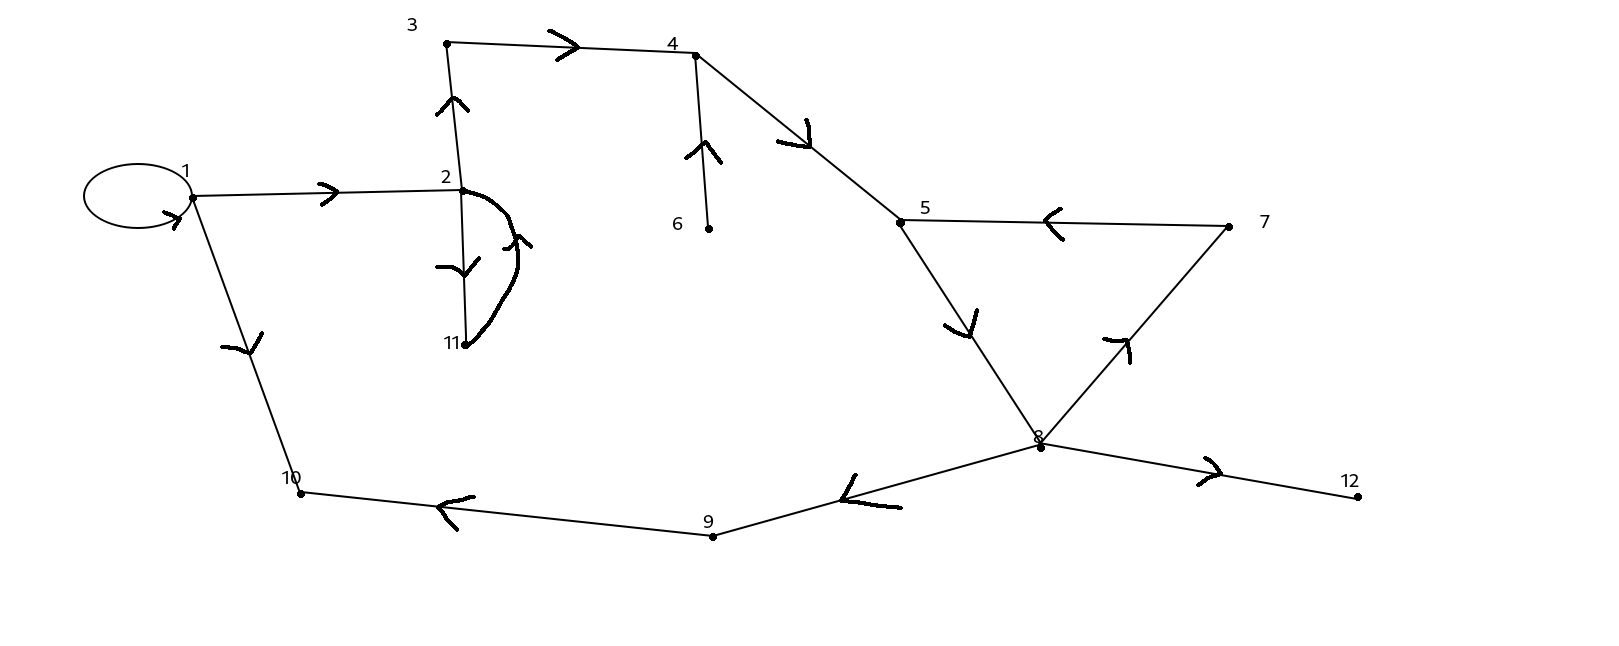
\includegraphics[bb=0 0 400 200]{pic/grafodirettoes.png}
        \begin{itemize}
          \item (2,11,2,3,4) e' un cammino diretto
          \item (1,2,3,4) e' un sentiero diretto
          \item (7,5,8,7,5,8,7) e' un cammino diretto chiuso
          \item (7,5,8,7) e' un ciclo diretto
          \item (2,11,2) e' un ciclo diretto
          \item (1,1) e' un ciclo diretto di lunghezza 1
          \item 4 e 9 sono comparabili
          \item 1 e 6 sono incomparabili
          \item (5,8,10) sono una catena
          \item (6,1) e' un anticatena
          \item (2,6,4) non e' ne una catena, ne un anticatena
          \item $d_+(5)=1$, $d_-(5)=2$
          \item $d_+(1)=3$, $d_-(1)=1$
          \item $d_+(12)=0$, $d_-(12)=1$
        \end{itemize}
        \subsection{Reti di communicazione}
        \subsection*{Definizioni}
        \begin{itemize}
          \item Una rete di communicazione e' una terna (R,I,O) dove R=(V,A) e' un grafo diretto
            $I \subseteq V$,$O\subseteq V$, $I \cap O =\o$ e $\mid I \mid =\mid O \mid=N$.
            Gli elementi di I si dicono nodi di input, gli elementi di O si dicono nodi di output
        \end{itemize}
        Sia (R,I,O) una rete di communicazioni
        \begin{itemize}
          \item Un problema di smistamento per la nostra rete di communicazione e' una permutazione $\pi \in S_N$. Sia $\pi \in S_N$
          \item Uno smistamento per $\pi$ e' una sequenza $(P_1,...,P_N)$ dove $P_j$ e' un cammino diretoo che va da $i_j$ a $o_{\pi(j)}$, $\forall j=1...N$ \\ 
            Dove $I=\{i_1,...,i_N\}$ e $O=\{o_1,...,o_N\}$
        \end{itemize}
        Sia $(P_1,...,P_n)$ un tale smistamento
        \begin{itemize}
          \item La latenza di $(P_1,...,P_N)$ e'
            \begin{equation*}
              max\{l(P_j):j=1,...,N\}
            \end{equation*}
          \item La congestione di $(P_1,...,P_N)$ e' 
            \begin{equation*}
              c(P_1,...,P_N)=max\{j\in N:x\in P_j\}
            \end{equation*}
        \end{itemize}
        \begin{flushleft}
          L insieme dei cammini che passano per un vertice e noi vogliamo il massimo
        \end{flushleft}
        Siano $x,y \in V$
        \begin{itemize}
          \item La distanza da x a y e' la lunghezza minima di un cammino drietto da x a y, scritto d(x,y). Se y non e raggiungibile da x allora scriveremo d(x,y)=$+\infty$
          \item Il diametro di (R,I,O) e'
            \begin{equation*}
              max\{d(i_j,o_k): 1\leq j,k\leq N\} 
            \end{equation*}
          \item La congestione di (R,I,O) e'
            \begin{equation*}
              max_{\pi \in S_N}\{min_{(P_1,...,P_N)}\{c(P_1,...,P_N)\} \to \quad \text{ scritto c(R,I,O)}
            \end{equation*}
        \end{itemize}
        \begin{flushleft}
          Sia (R,I,O) una rete di communicazione 
        \end{flushleft}
        \begin{flushleft}
          Def i vertici di (R,I,O) si dicono anche switch 
        \end{flushleft}
        \begin{flushleft}
          Sia $v\in V$
        \end{flushleft}
        \begin{flushleft}
          Def: La grandezza di v e' $d_+(v),d_-(v)$
        \end{flushleft}
        \begin{flushleft}
          Si dice anche che v e' uno ($d_+(v),d_-(v)$)-switch
        \end{flushleft}
        \begin{flushleft}
          L'obbiettivo delle rete di communicazioni
        \end{flushleft}
        \begin{enumerate}
          \item congestione bassa
          \item pochi switch
          \item avere switch piccoli
        \end{enumerate}
        \subsection*{Grafi/Reti di communicazione notevoli}
        \begin{flushleft}
          La griglia $G_5$ e'
        \end{flushleft}
        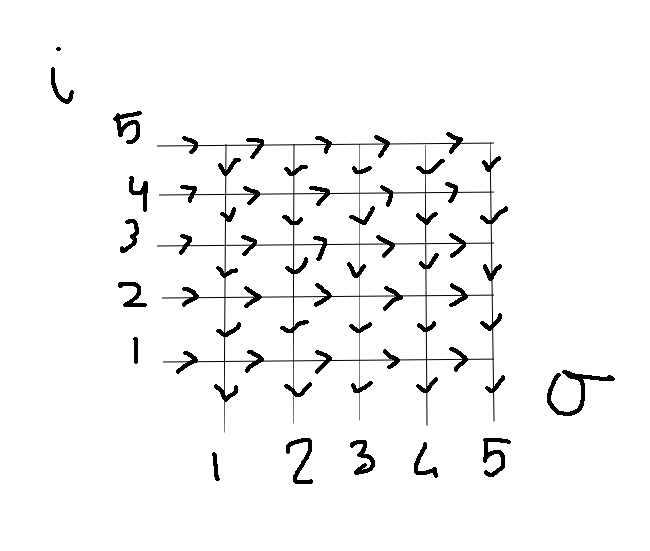
\includegraphics[bb=0 0 120 120]{pic/griglia5.png}
        \subsubsection{Teorema}
        \begin{flushleft}
          Sia $n\in \mathbb{P}$. Allora
        \end{flushleft}
        \begin{equation*}
          c(G_N)=2
        \end{equation*}
        \begin{flushleft}
          Dimostrazione: e' chiaro che la congestione non puo' essere 1 ($c(G_N)>1$ se $\pi \in S_N$)
        \end{flushleft}
        \begin{flushleft}
          e' tale che $\pi(1)=n$ e $\pi(n)=1$ e se $(P_1,...,P_n)$ e' uno smistamento per $\pi \Rightarrow P_1 \cap P_n \neq \o$
        \end{flushleft}
        \begin{flushleft}
          Sia $\pi \in S_N$ e sia x il della stessa riga di $i_a$ e nella stessa colonna di $o_b$. Dove $a,b\in [n]$. Poniamo (a,b)=x.
        \end{flushleft}
        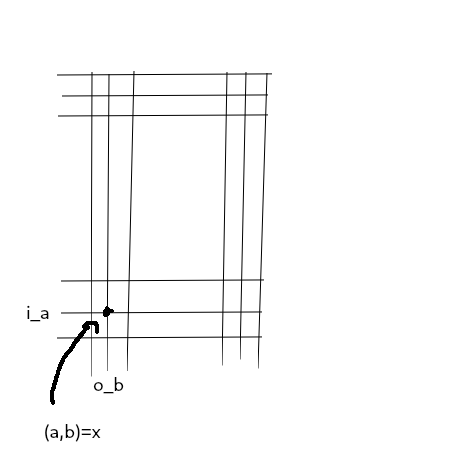
\includegraphics[bb=0 0 150 150]{pic/dimostrazioneXvertice.png}
        \begin{flushleft}
          Definiamo uno smistamento $(P_1,...,P_n)$ in questo modo $P_j$ segue la riga j-esima fino alla colonna $\pi(j)$-esima $\forall j=1...n$
        \end{flushleft}
        \begin{flushleft}
          Allora $c(G_N)=2$
        \end{flushleft}
        \begin{flushleft}
          Sia $P_j$ un cammino tale che $(a,b)\in P_j \Rightarrow$ o j=a oppure $\pi(j)=b \Rightarrow$ j=a o j=$\pi^{-1}(b) \Rightarrow$ al piu' possibilita' per $P_j$ quindi $c(P_1,...,P_n)=2$
        \end{flushleft}
        Sia $k\in \mathbb{P}$
        \begin{flushleft}
          Def: la farfalla $F_k$ e' definita induttivamente come segue
        \end{flushleft}
        \begin{flushleft}
          $F_1=$
        \end{flushleft}
        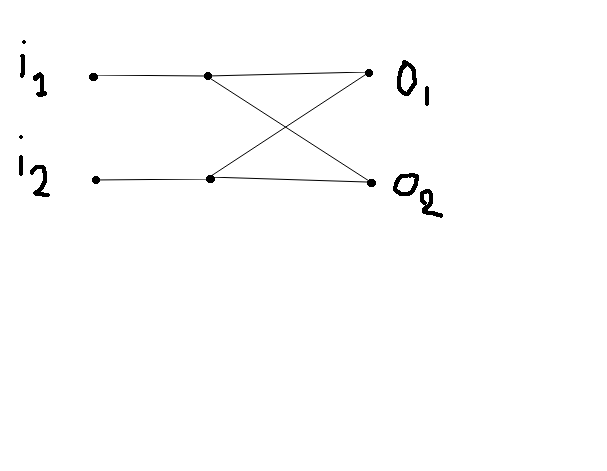
\includegraphics[bb=0 0 200 200]{pic/f1farfalla.png}
        \begin{flushleft}
          $F_2=$
        \end{flushleft}
        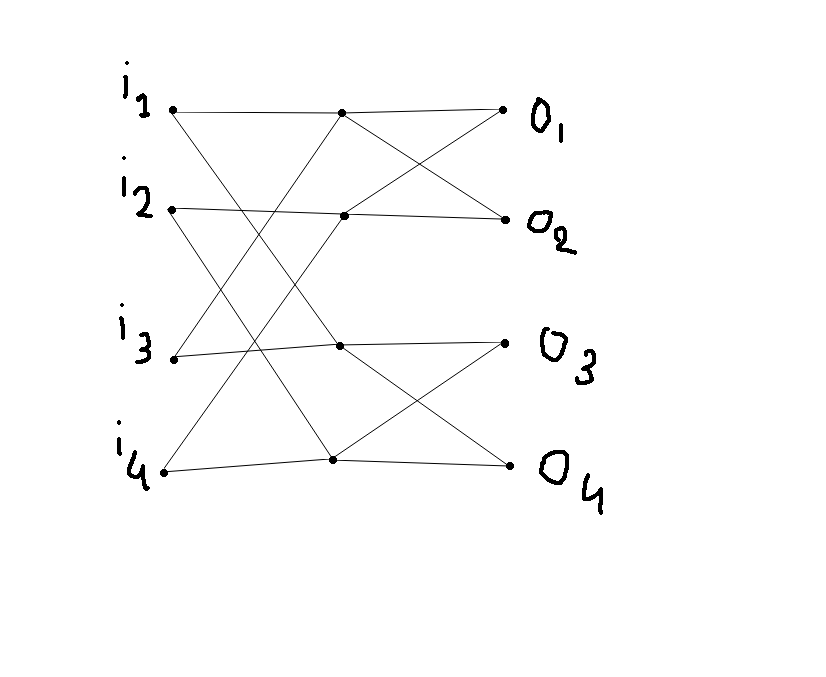
\includegraphics[bb=0 0 200 200]{pic/f2farfalla.png}
        \begin{flushleft}
          Dato un qualsiasi nodo di input e di output c'e' un solo cammino che li collega
        \end{flushleft}
        \begin{flushleft}
          Formalmente: $F_k=(R,I,O)$ dove $R=(V,E)$ dove 
        \end{flushleft}
        \begin{equation*}
          V=\{(\epsilon_1,...,\epsilon_k;i) \quad \text{ e } \quad [0,1]x[k+1]\}
        \end{equation*}
        e
        \begin{equation*}
          (\epsilon_1,...,\epsilon_k;i) \to (\eta_1,...,\eta_k;j)
        \end{equation*}
        \begin{flushleft}
          Si collegano se solo se
        \end{flushleft}
        \begin{equation*}
          j=i+1 \quad \text{ e } \quad \epsilon_2=\eta_2 \quad \forall r\in [k+1] / \{i\}
        \end{equation*}
        \begin{flushleft}
          Oss: c'e' un solo sentiero diretto da un qualsiasi nodo di input a qualsiasi nodo di output
        \end{flushleft}
        E.g
        \begin{equation*}
          i_{1001}=(1001;1)\to (1001;2) \to (1101;3) \to (1101;4) \to (1101;5)=o_{1101}
        \end{equation*}
        \subsubsection{Teorema}
        \begin{flushleft}
          La congestione della farfalla e'
        \end{flushleft}
        \begin{equation*}
          c(F_k)=\begin{cases}
            2^{\frac{k}{2}} \quad \text{ se k e' pari }\\ 
            2^{\frac{k-1}{2}} \quad \text{  se k e' dispari }
          \end{cases}
        \end{equation*}
        \begin{flushleft}
          Dimostrazione (idea) 
        \end{flushleft}
        \begin{flushleft}
          Sia $\pi \in S_n$ ($N=2^k$) e sia $(P_1,...,P_n)$ uno smistamento per $\pi$. Sia
        \end{flushleft}
        \begin{equation*}
          (\epsilon_1,...,\epsilon_k;i)\in V
        \end{equation*}
        \begin{flushleft}
          Sia $P_j$ tale che $x\in P_j$. Allora il nodo di output di $P_j$ e' della forma
        \end{flushleft}
        \begin{equation*}
          (\epsilon_1,...,\epsilon_{i-1},x_i,...,x_k,k+1)
        \end{equation*}
        \begin{flushleft}
          $\Rightarrow 2^{k-i+1}$ possibilita'. Similmente il nodo di input di $P_j$ e' della forma
        \end{flushleft}
        \begin{equation*}
          (x_1,...,x_{i-1},\epsilon_i,...,\epsilon_k;j)
        \end{equation*}
        \begin{flushleft}
          $\Rightarrow 2^{i-1}$ sono 
        \end{flushleft}
        \begin{equation*}
          min\{2^{i-1},2^{k-i+1}\}
        \end{equation*}
        \begin{flushleft}
          possibilita' per $P_j$ ma
        \end{flushleft}
        \begin{equation*}
          min\{2^{i-1},2^{k-i+1}\}\leq \begin{cases}
            2^{\frac{k}{2}} \quad \text{ se k e' pari }\\ 
            2^{\frac{k-1}{2}} \quad \text{  se k e' dispari }
          \end{cases}
        \end{equation*}
        \begin{flushleft}
          che equivale a dire
        \end{flushleft}
        \begin{equation*}
          min\{i-1,k-i+1\}\leq \begin{cases}
            \frac{k}{2} \quad \text{ se k e' pari }\\ 
            \frac{k-1}{2} \quad \text{  se k e' dispari }
          \end{cases}
        \end{equation*}
        Concludendo
        \begin{center}
          \begin{tabular}{ | m{1cm} | m{3cm}| m{3cm} | m{9em} | m{3cm} |} 
            \hline
            Rete & numero di nodi& numero di terminali& congestione& grandezza degli switch\\ 
            \hline
            $G_N$ & $N(N+2)$ & N& 2& 2x2\\ 
            \hline
            $F_k$ & $N(log_2(N)+1)$ & N (=$2^k$)& $\sqrt{N}$ se k e' pari,\quad $\sqrt{\frac{N}{2}}$ se k e' dispari& 2x2\\ 
            \hline
          \end{tabular}
        \end{center}
        \subsection{Orari Paralleli}
        \begin{flushleft}
          Sia D=(V,A) un grafo diretto
        \end{flushleft}
        \begin{flushleft}
          Def: un orario parallelo per D e' una partizione $\{B_0,B_1,...,B_k\}$ di v tale che 
        \end{flushleft}
        \begin{equation*}
          0 \leq i < j \leq k \Rightarrow \begin{cases}
            \text{nessun vertice di $B_i$} \\ 
            \text{e' raggiungibile da alcun vertice di $B_j$}
          \end{cases}
        \end{equation*}
        \begin{flushleft}
          $max\{\mid B_0\mid ,...,\mid B_k\mid \}$ si dice il numero di processori del nostro orario parallelo,
          gli elementi di $B_i$ si dicono il passo i-esimo dell'orario parallelo
        \end{flushleft}
        Sia $x \in V$
        \begin{flushleft}
          Def: un sentiero critico per x e' un sentiero diretto ($x_0,x_1,...,x_r$) in D. Tale che $x_r=x$ e se ($y_0,y_1,...,y_s$) e' 
          un altro sentiero tale che $y_s=x\Rightarrow r \geq s$
          (il piu' lungo sentiero che finisce in x)
        \end{flushleft}
        \begin{flushleft}
          Def: La profondita' di x, scritto dp(x) e' la lunghezza di un sentiero critico per x
        \end{flushleft}

      \end{document}
